%%%%%%%%%%%%%%%%%%%%%%%%%%%%%%%%%%%%%%%%%%  不使用 authblk 包制作标题  %%%%%%%%%%%%%%%%%%%%%%%%%%%%%%%%%%%%%%%%%%%%%%
%-------------------------------PPT Title-------------------------------------
\title{数据驱动视野下的材料设计}
%-----------------------------------------------------------------------------

%----------------------------Author & Date------------------------------------
%\author[\textrm{Jun\_Jiang}]{姜\;\;骏\inst{}} %[]{} (optional, use only with lots of authors)
%% - Give the names in the same order as the appear in the paper.
%% - Use the \inst{?} command only if the authors have different
%%   affiliation.
\institute[BCC]{\inst{}%
%\institute[Gain~Strong]{\inst{}%
\vskip 0pt 北京市计算中心有限公司}
%\vskip -20pt {\large 格致斯创~科技}}
\date[\today] % (optional, should be abbreviation of conference name)
{	%{\fontsize{6.2pt}{4.2pt}\selectfont{\textcolor{blue}{E-mail:~}\url{jiangjun@bcc.ac.cn}}}
\vskip 45 pt {\fontsize{8.2pt}{6.2pt}\selectfont{%北京科技大学% 报告地点
	\vskip 5 pt \textrm{2024.06}}}
}

%% - Either use conference name or its abbreviation
%% - Not really information to the audience, more for people (including
%%   yourself) who are reading the slides onlin%%   yourself) who are reading the slides onlin%%   yourself) who are reading the slides onlineee
%%%%%%%%%%%%%%%%%%%%%%%%%%%%%%%%%%%%%%%%%%%%%%%%%%%%%%%%%%%%%%%%%%%%%%%%%%%%%%%%%%%%%%%%%%%%%%%%%%%%%%%%%%%%%%%%%%%%%

\subject{}
% This is only inserted into the PDF information catalog. Can be left
% out.
%\maketitle
\frame
{
%	\frametitle{\fontsize{9.5pt}{5.2pt}\selectfont{\textcolor{orange}{“高通量并发式材料计算算法与软件”年度检查}}}
\titlepage
}
%-----------------------------------------------------------------------------

%------------------------------------------------------------------------------列出全文 outline ---------------------------------------------------------------------------------
%\section*{}
%\frame[allowframebreaks]
%{
%  \frametitle{Outline}
%%  \frametitle{\textcolor{mycolor}{\secname}}
%  \tableofcontents%[current,currentsection,currentsubsection]
%}
%%在每个section之前列出全部Outline
%%类似的在每个subsection之前列出全部Outline是\AtBeginSubsection[]
%\AtBeginSection[]
%{
%  \frame<handout:0>%[allowframebreaks]
%  {
%    \frametitle{Outline}
%%全部Outline中,本部分加亮
%    \tableofcontents[current,currentsection]
%  }
%}

%-----------------------------------------------PPT main Body------------------------------------------------------------------------------------
\small
%\section{引言}
\frame
{
	\frametitle{科学研究的范式变更}
\begin{figure}[h!]
\vspace*{-0.28in}
\centering
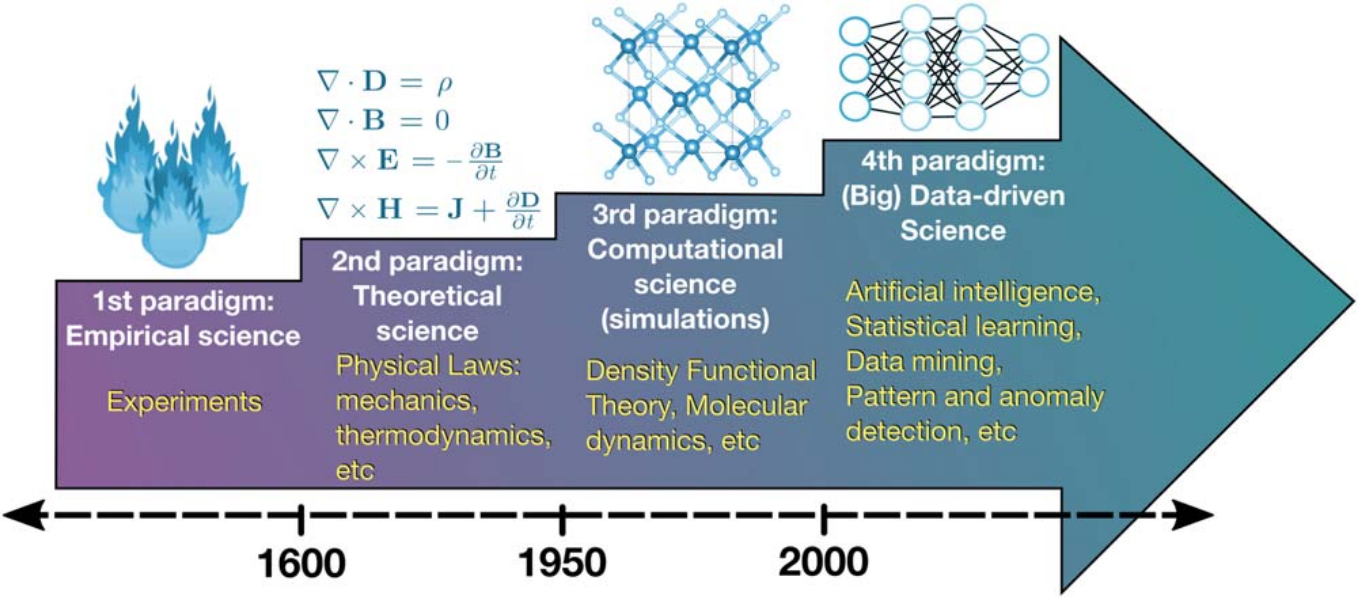
\includegraphics[height=2.00in,width=4.15in]{Figures/Four_Model_3.png}
%\caption{\tiny \textrm{Pseudopotential for metallic sodium, based on the empty core model and screened by the Thomas-Fermi dielectric function.}}%(与文献\cite{EPJB33-47_2003}图1对比)
\label{Four_Model}
\end{figure}
\begin{minipage}[b]{0.48\textwidth}
 {\fontsize{9.5pt}{6.0pt}\selectfont\begin{itemize}%[+-| alert@+>]
	 \setlength{\itemsep}{6pt}
 \item 逐步趋于理性
 \item 逐步趋于复杂
 \end{itemize}}
\end{minipage}
\hfill
\begin{minipage}[b]{0.48\textwidth}
 {\fontsize{9.5pt}{6.0pt}\selectfont\begin{itemize}%[+-| alert@+>]
	 \setlength{\itemsep}{6pt}
 \item 逐步趋于抽象
 \item 逐步趋于深刻
 \end{itemize}}
\end{minipage}
}

\frame
{
	\frametitle{材料基因工程的理念}
\begin{minipage}[c]{0.31\textwidth}
\begin{itemize}%[+-| alert@+>]
\vspace*{-1.85in}
 {\fontsize{8.5pt}{6.0pt}\selectfont
	 \setlength{\itemsep}{10pt}
 \item 变革研发模式,计算-实验-理论-数据科学相融合: 高效、低耗按需设计
 \item 数据驱动的材料创新平台主要面向复杂材料的模拟}
 \end{itemize}
\end{minipage}
\hfill
\begin{minipage}[b]{0.67\textwidth}
\begin{figure}[h!]
%\vspace*{-0.25in}
\centering
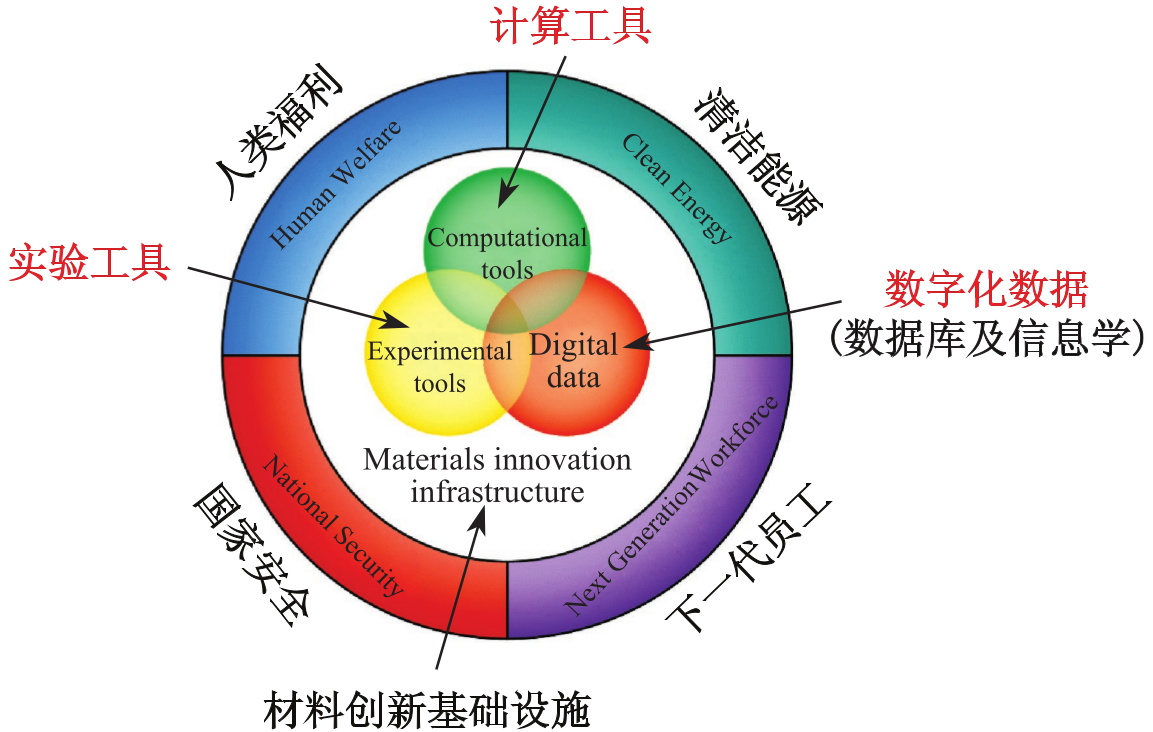
\includegraphics[height=1.60in,width=2.55in]{Figures/Mat_Geno_Ene-1.png}
%\caption{\tiny \textrm{Pseudopotential for metallic sodium, based on the empty core model and screened by the Thomas-Fermi dielectric function.}}%(与文献\cite{EPJB33-47_2003}图1对比)
\label{Mater_Genome}
\end{figure}
\end{minipage}
\vskip 5pt
\textcolor{magenta}{本单位参与国家重点研发计划项目}
\begin{itemize}
	\setlength{\itemsep}{3pt}
	\item {\fontsize{8.2pt}{5.0pt}\selectfont{“\textcolor{blue}{高通量并发式材料计算算法和软件}”}}{\fontsize{6.2pt}{4.2pt}\selectfont{(编号:~\textrm{2017YFB0701500})}}
		%{\fontsize{8.2pt}{6.2pt}\selectfont{(本单位任务责任人)}}
	\item {\fontsize{8.2pt}{5.0pt}\selectfont{“\textcolor{blue}{材料高通量计算/实验平台数据自动汇交技术}”}}{\fontsize{6.2pt}{4.2pt}\selectfont{(编号:~\textrm{2017YFB0704302})}}
		%{\fontsize{8.2pt}{6.2pt}\selectfont{(参与)}}
	\item {\fontsize{8.2pt}{5.0pt}\selectfont{“\textcolor{blue}{国家材料基因工程数据管理与数据服务技术平台}”}}{\fontsize{6.2pt}{4.2pt}\selectfont{(编号:~\textrm{2018YFB0704300})}}
		%{\fontsize{8.2pt}{6.2pt}\selectfont{(参与)}}
\end{itemize}
}

\frame
{
	\frametitle{材料设计的基本思想}
\begin{figure}[h!]
\vspace*{-0.20in}
\centering
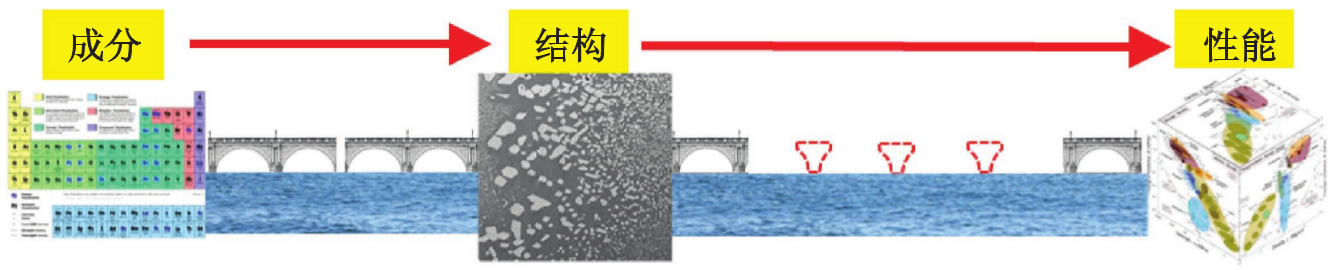
\includegraphics[height=0.70in,width=3.75in]{Figures/MGE-2.png}
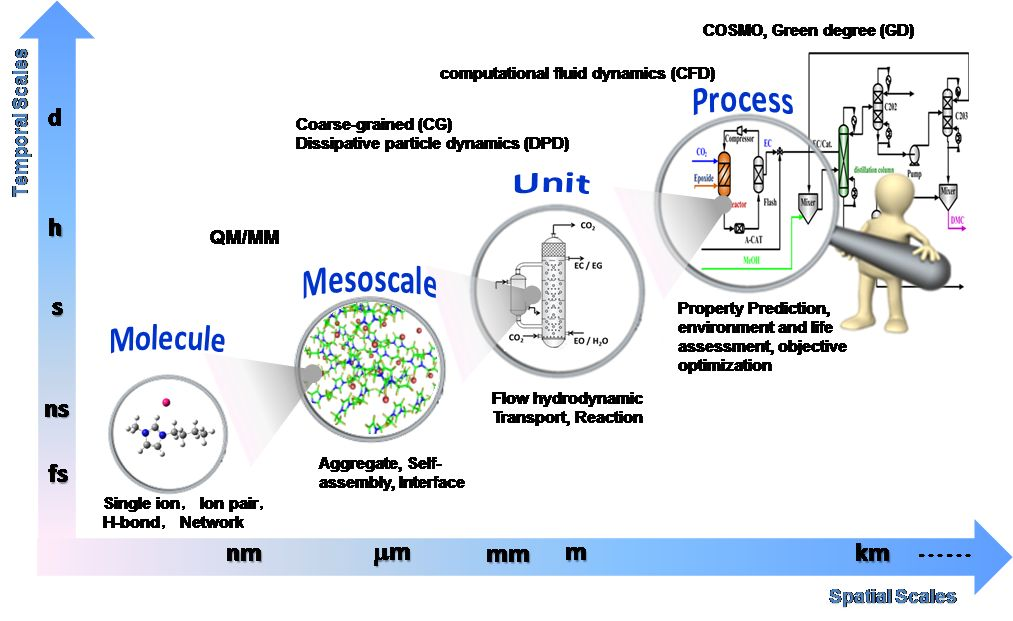
\includegraphics[height=1.90in,width=3.75in,viewport=-120 0 775 480,clip]{Figures/Multi_Scale-2.jpeg}
%\caption{\tiny \textrm{Pseudopotential for metallic sodium, based on the empty core model and screened by the Thomas-Fermi dielectric function.}}%(与文献\cite{EPJB33-47_2003}图1对比)
\label{MGE}
\end{figure}
{\fontsize{7.2pt}{5.0pt}\selectfont{还原论\textrm{(reductionism)}:\\\textcolor{red}{复杂系统表现的性质(现象),可归结为最基本的组成单元和决定单元行为的基本规律}}}
}

\frame
{
	\frametitle{跨尺度计算:~微观尺度的尝试}
	\textcolor{blue}{将复杂还原为简单的目的是从简单重建复杂}
\begin{itemize}
	\item 量子力学:~原子间相互作用用原子核与电子运动(定量)描述
\begin{figure}[h!]
\vspace*{-0.08in}
\centering
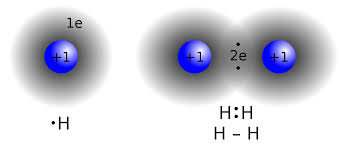
\includegraphics[height=1.05in,width=2.10in,viewport=0 0 350 160,clip]{Figures/H-bonding.jpeg}
%\caption{\tiny \textrm{Schematic illustration of modeling a simple alloy from atoms.}}%(与文献\cite{EPJB33-47_2003}图1对比)
\label{H-bondinfg}
\end{figure}
	\item 分子动力学:~原子间相互作用用力场函数(唯象)描述
\begin{figure}[h!]
\vspace*{-0.10in}
\centering
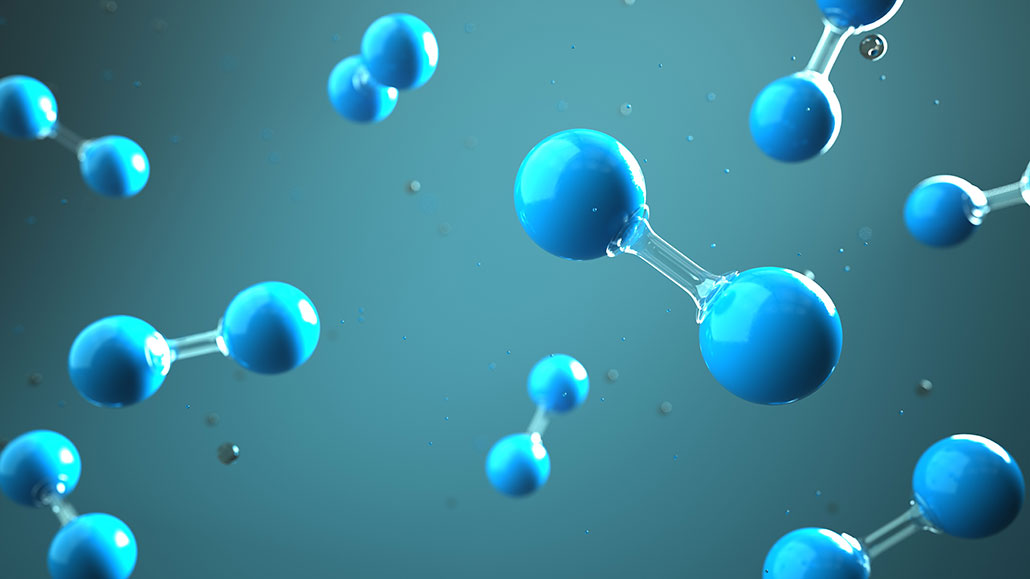
\includegraphics[height=1.05in,width=2.10in,viewport=0 0 1050 650,clip]{Figures/Chemical_Bonding_2.jpg}
%\caption{\tiny \textrm{Schematic illustration of modeling a simple alloy from atoms.}}%(与文献\cite{EPJB33-47_2003}图1对比)
\label{Chemical_Bonding}
\end{figure}
\end{itemize}

}

\frame
{
	\frametitle{跨尺度计算:~微观尺度的尝试}
%	\textcolor[rgb]{0.00, 1.00, 0.00}{还原论\textrm{(reductionism)}}:~将复杂还原为简单,然后再从简单重建复杂\\
\begin{itemize}
	\item 在每一还原层次,系统特征的空间尺度迅速变小,特征的能量/时间尺度急剧升高
\begin{figure}[h!]
\vspace*{-0.08in}
\centering
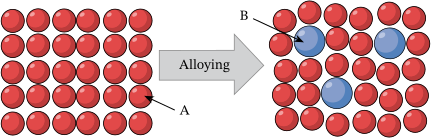
\includegraphics[height=1.12in,width=3.85in,viewport=0 0 365 115,clip]{Figures/Alloy_modeling.png}
\caption{\tiny \textrm{Schematic illustration of modeling a simple alloy from atoms.}}%(与文献\cite{EPJB33-47_2003}图1对比)
\label{Alloy_modeling}
\end{figure}
	\item 数值计算的困难程度随着体系尺度的增大而指数增加,从理论上准确预测大量粒子组成体系的性质难度极大
\end{itemize}
}

\frame
{
	\frametitle{跨尺度计算:~微观尺度的尝试}
\begin{figure}[h!]
\vspace*{-0.15in}
\centering
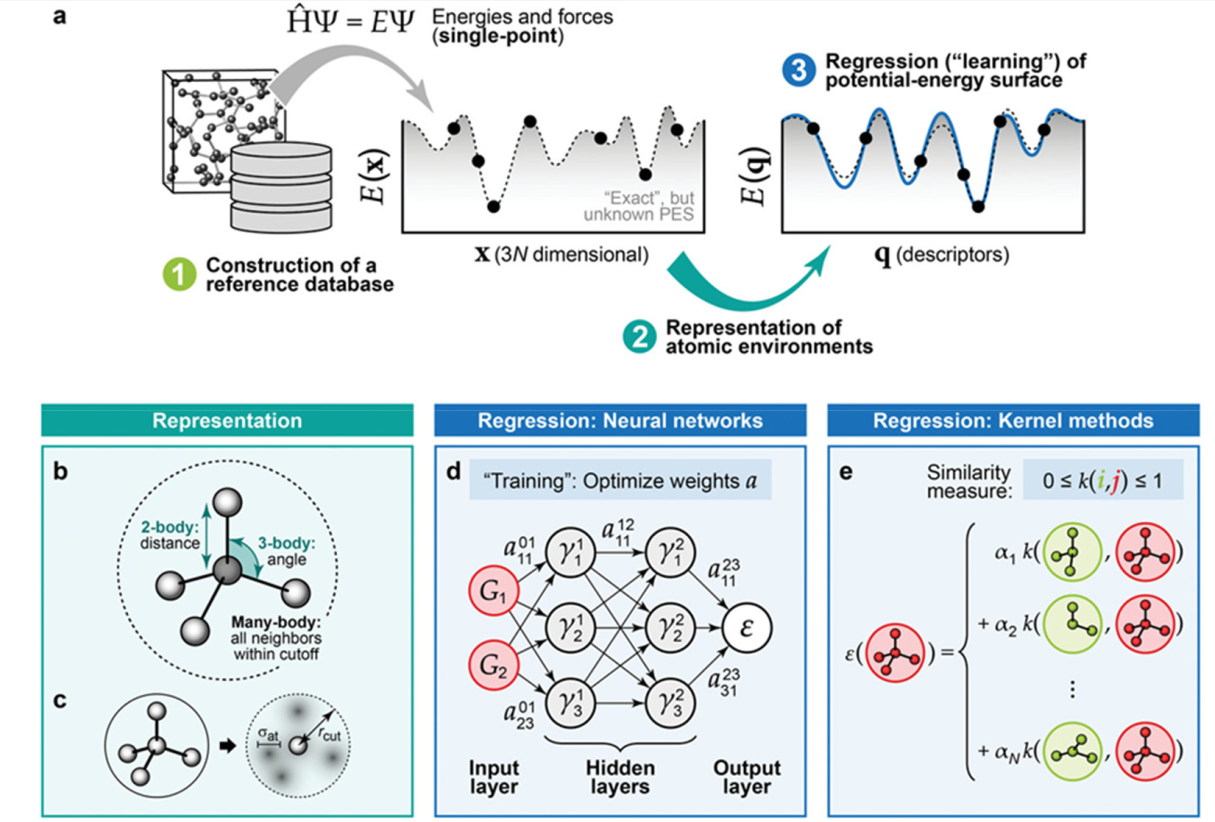
\includegraphics[height=2.25in,width=3.65in,viewport=0 0 1215 822,clip]{Figures/Schematic-illustration-machine_learning_algorithm-to-find-the-relationship-of-the-atomic_configuration-and-energy.png}
%\caption{\tiny \textrm{Schematic illustration of modeling a simple alloy from atoms.}}%(与文献\cite{EPJB33-47_2003}图1对比)
\label{Schematic-illustration-machine_learning_algorithm-to-find-the-relationship-of-the-atomic_configuration-and-energy}
\end{figure}
机器学习方法:~挖掘复杂体系原子结构与(量子力学)能量内在关联
}

\frame
{
	\frametitle{跨尺度计算的主要困难:~\textcolor[rgb]{1.00, 0.20 0.20}{多者异也}}
		\begin{itemize}
		\item 面向尺度和复杂性:~\textrm{Philip~W.~Anderson}提出``多者异也''~\textrm{(\textcolor[rgb]{0.00, 0.00, 1.00}{More is different})}的思想:~
\vskip 3pt
{\fontsize{7.2pt}{5.0pt}\selectfont{复杂体系在每一不同的聚集层次,都会呈现出许多预想不到的全新复杂物理性质,这些性质已经远超出组成基元的物理学规律}}
\begin{figure}[h!]
\vspace*{-0.05in}
\centering
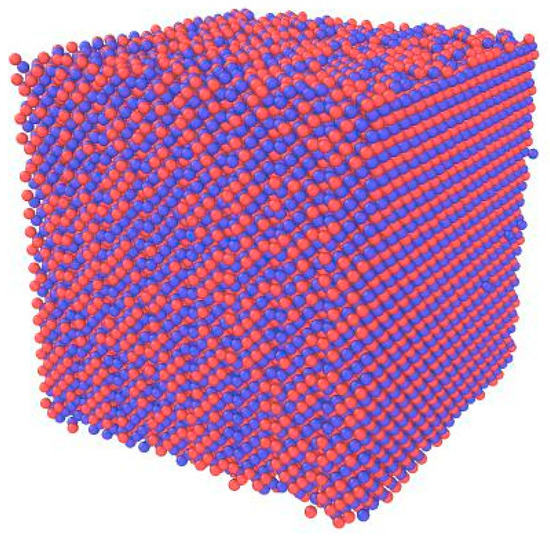
\includegraphics[height=1.35in,width=1.65in,viewport=0 0 425 420,clip]{Figures/Ti-Al_alloy_model.jpg}
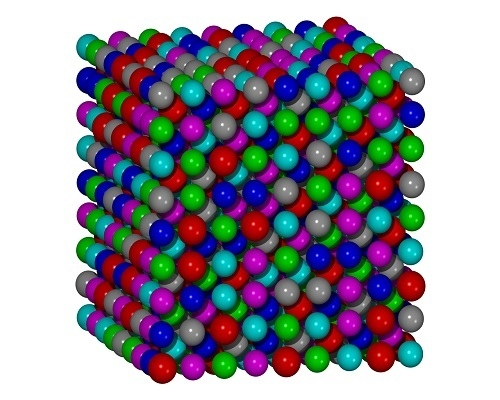
\includegraphics[height=1.35in,width=1.65in,viewport=55 10 335 305,clip]{Figures/high-entropy_alloys.jpg}
%\caption{\tiny \textrm{Pseudopotential for metallic sodium, based on the empty core model and screened by the Thomas-Fermi dielectric function.}}%(与文献\cite{EPJB33-47_2003}图1对比)
\label{Flow-of-multi_scale-modelling}
\end{figure}
	\end{itemize}
	{\fontsize{7.2pt}{5.0pt}\selectfont{演生论\textrm{(emergence)}:\\
	\textcolor{red}{在每一个复杂性的发展层次中,都会呈现出全新的物理概念、物理定律和物理原理}}}
}

\frame
{
	\frametitle{数据驱动:~跨尺度计算的曙光}
\begin{figure}[h!]
\vspace*{-0.15in}
\centering
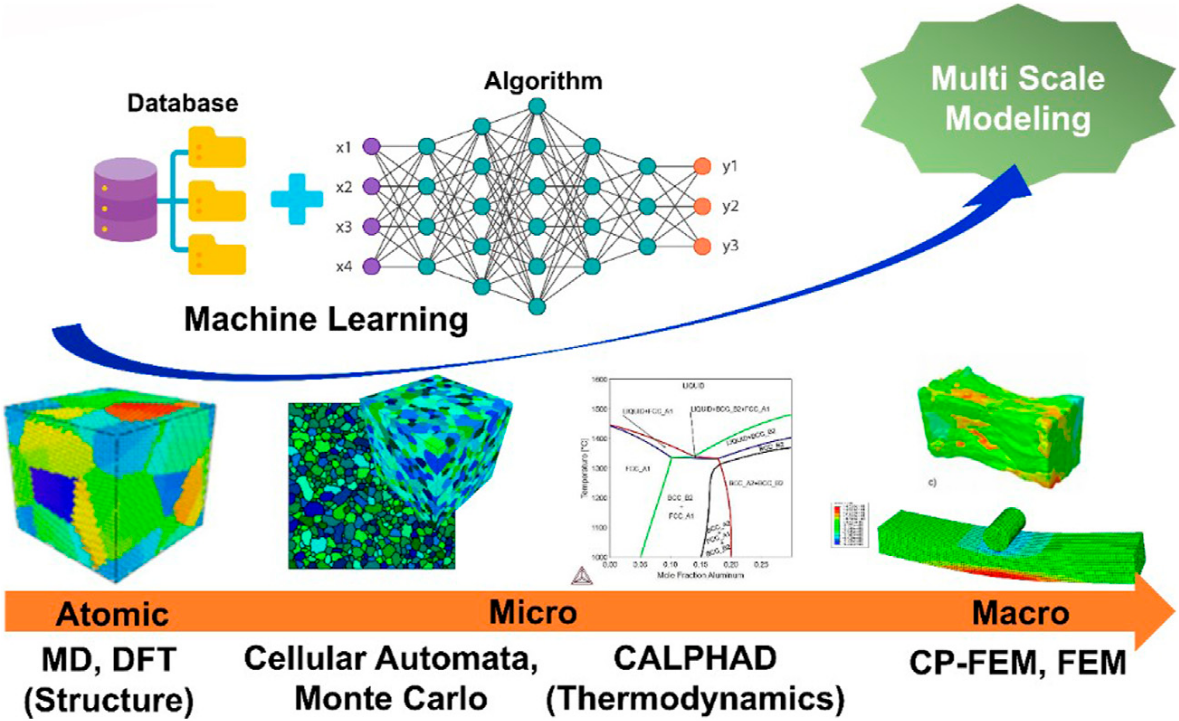
\includegraphics[height=2.65in,width=4.05in,viewport=0 0 1179 721,clip]{Figures/Schematic_flow-of-multi_scale-modelling.png}
%\caption{\tiny \textrm{Pseudopotential for metallic sodium, based on the empty core model and screened by the Thomas-Fermi dielectric function.}}%(与文献\cite{EPJB33-47_2003}图1对比)
\label{Data_for-Machine-Leaning}
\end{figure}
}

%\frame
%{
%	\frametitle{计算材料数据}
%	现有材料数据内容
%\begin{figure}[h!]
%\vspace*{-0.15in}
%\centering
%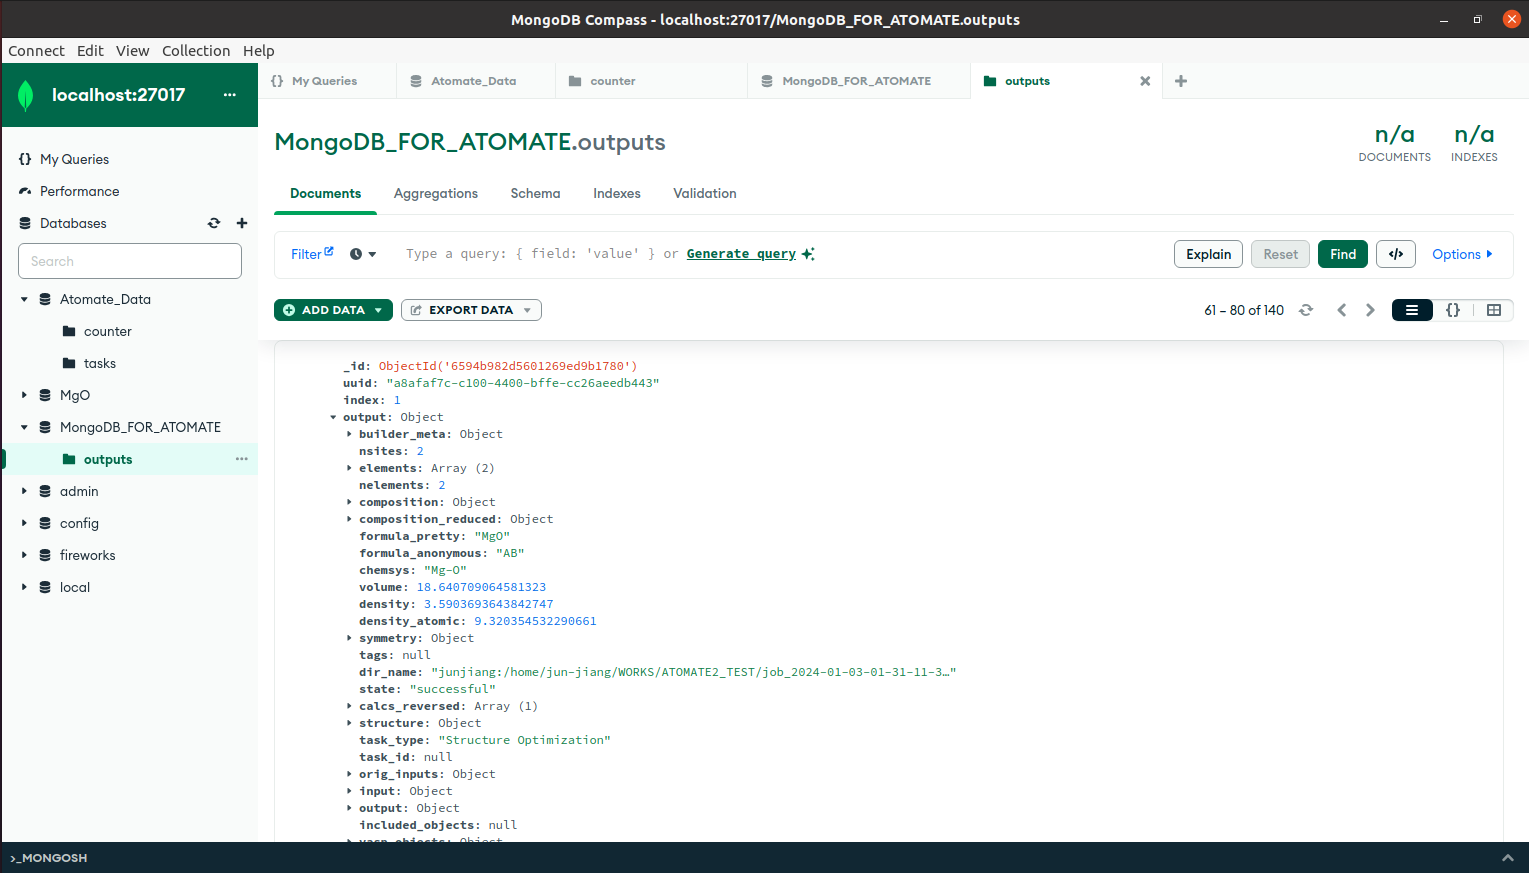
\includegraphics[height=2.35in,width=4.05in,viewport=0 0 1529 873,clip]{Figures/Database_Materials.png}
%%\caption{\tiny \textrm{Pseudopotential for metallic sodium, based on the empty core model and screened by the Thomas-Fermi dielectric function.}}%(与文献\cite{EPJB33-47_2003}图1对比)
%\label{DataBase_Materials}
%\end{figure}
%}
%
\frame
{
	\frametitle{计算材料数据}
	现有材料数据内容\\
	\begin{tikzpicture}[
    box/.style={rectangle,draw,fill=darkgray!20,node distance=1cm,text width=15em,text centered,rounded corners,minimum height=2em,thick},]
\node at (-5,0) (Figure){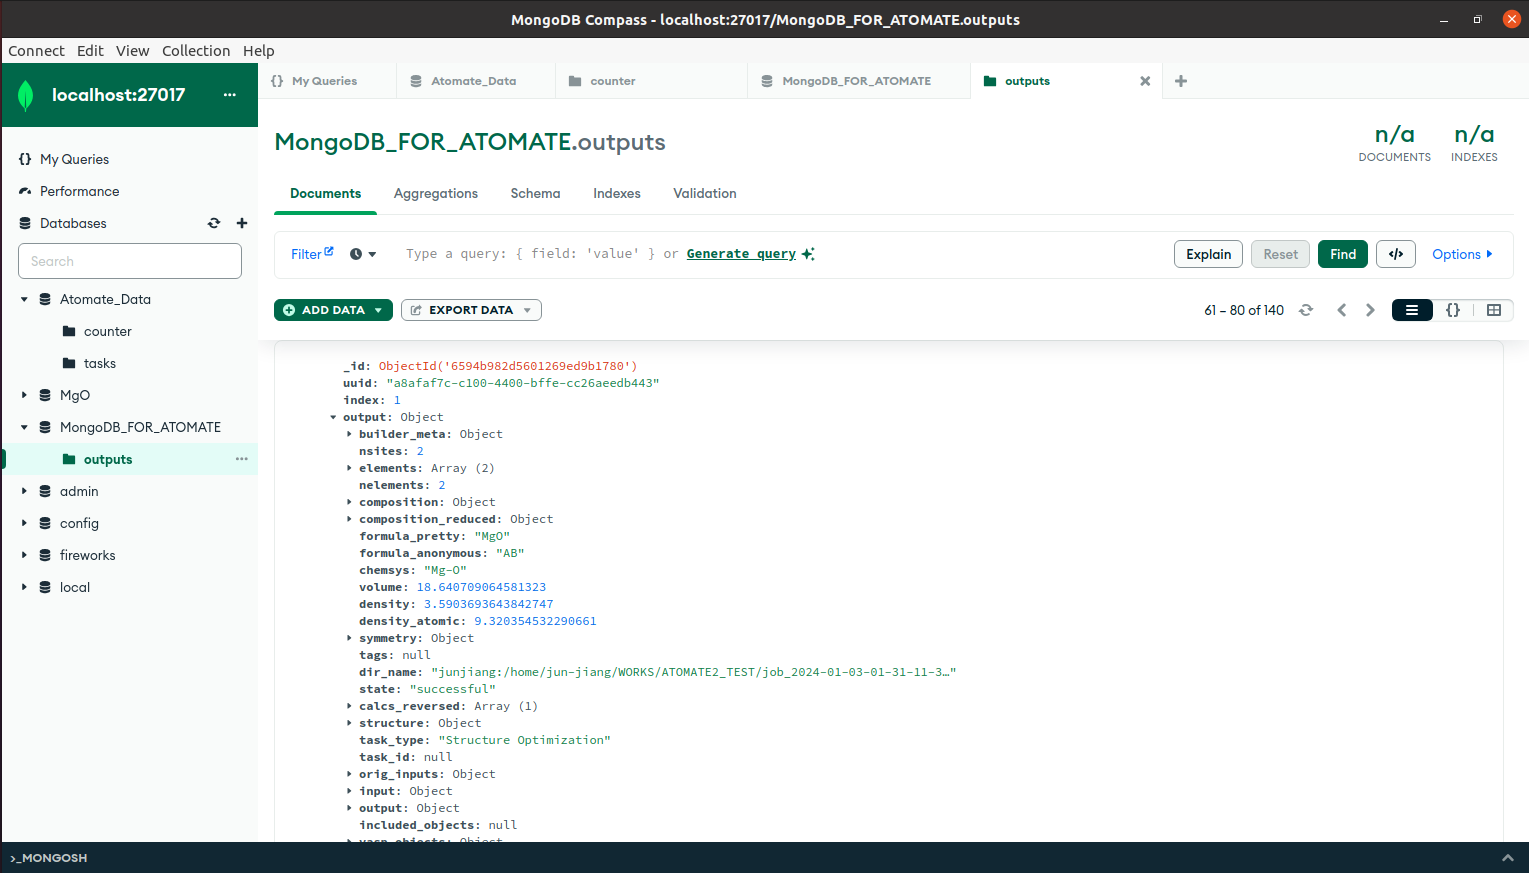
\includegraphics[height=2.35in,width=4.05in,viewport=0 0 1529 873,clip]{Figures/Database_Materials.png}};
\node[rectangle,draw=red, dashdotted, inner sep=1em] at (-1.75, 0.7) (enclosure) {};
%\caption{\tiny \textrm{Pseudopotential for metallic sodium, based on the empty core model and screened by the Thomas-Fermi dielectric function.}}%(与文献\cite{EPJB33-47_2003}图1对比)
\end{tikzpicture}
}

\frame
{
	\frametitle{计算材料数据:~计算流程}
	现有材料数据计算流程
\begin{figure}[h!]
\vspace*{-0.15in}
\centering
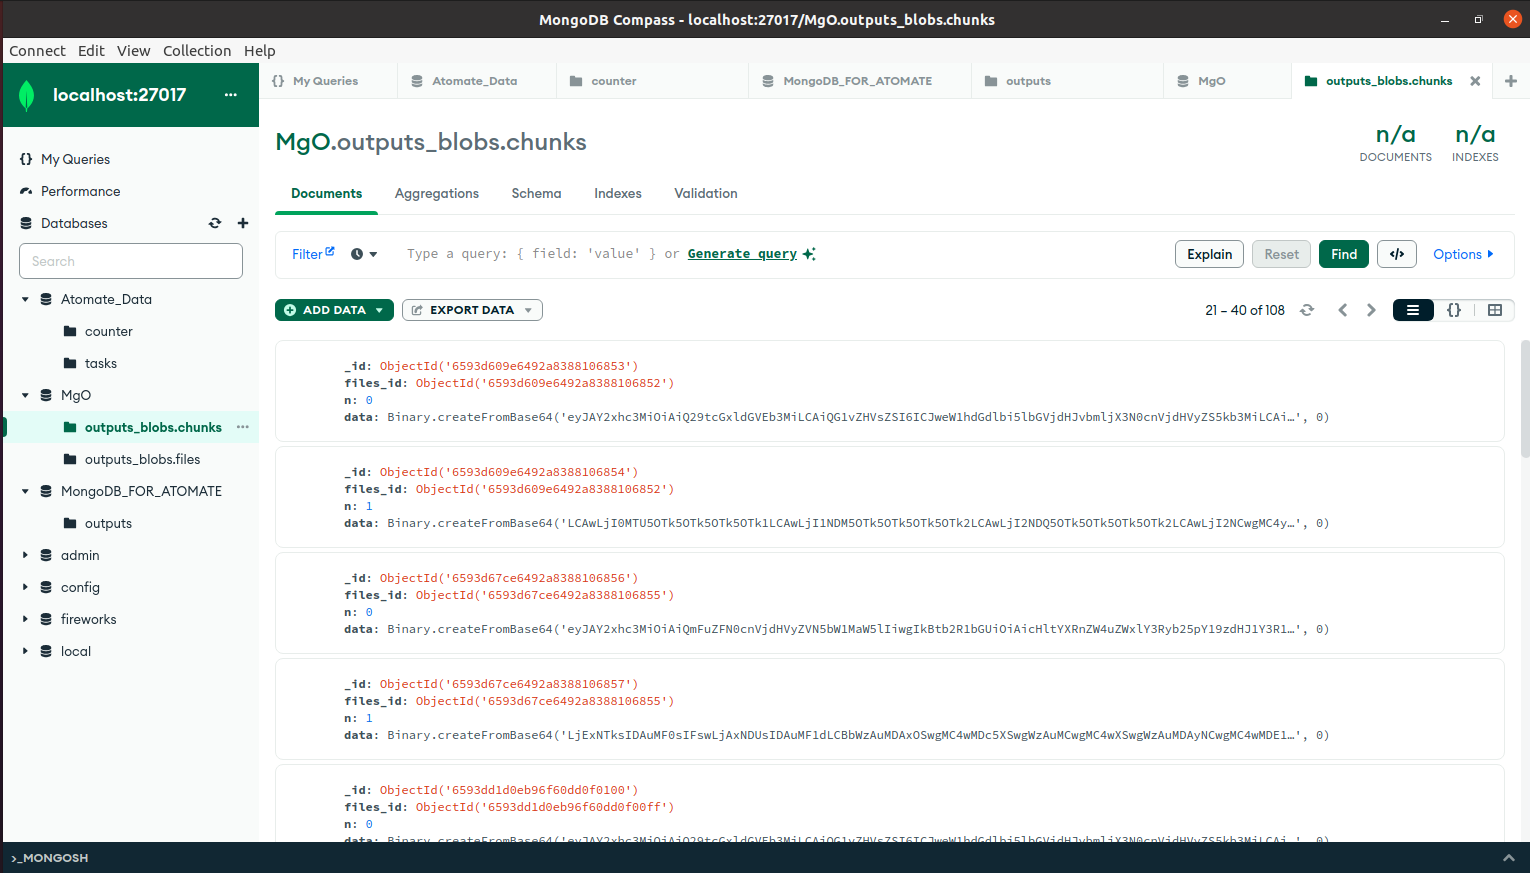
\includegraphics[height=2.35in,width=4.05in,viewport=0 0 1530 873,clip]{Figures/Database_Materials-Flow.png}
%\caption{\tiny \textrm{Pseudopotential for metallic sodium, based on the empty core model and screened by the Thomas-Fermi dielectric function.}}%(与文献\cite{EPJB33-47_2003}图1对比)
\label{DataBase_Materials-Flow}
\end{figure}
}

\frame
{
	\frametitle{计算材料数据:~数据库}
\begin{figure}[h!]
\vspace*{-0.15in}
\centering
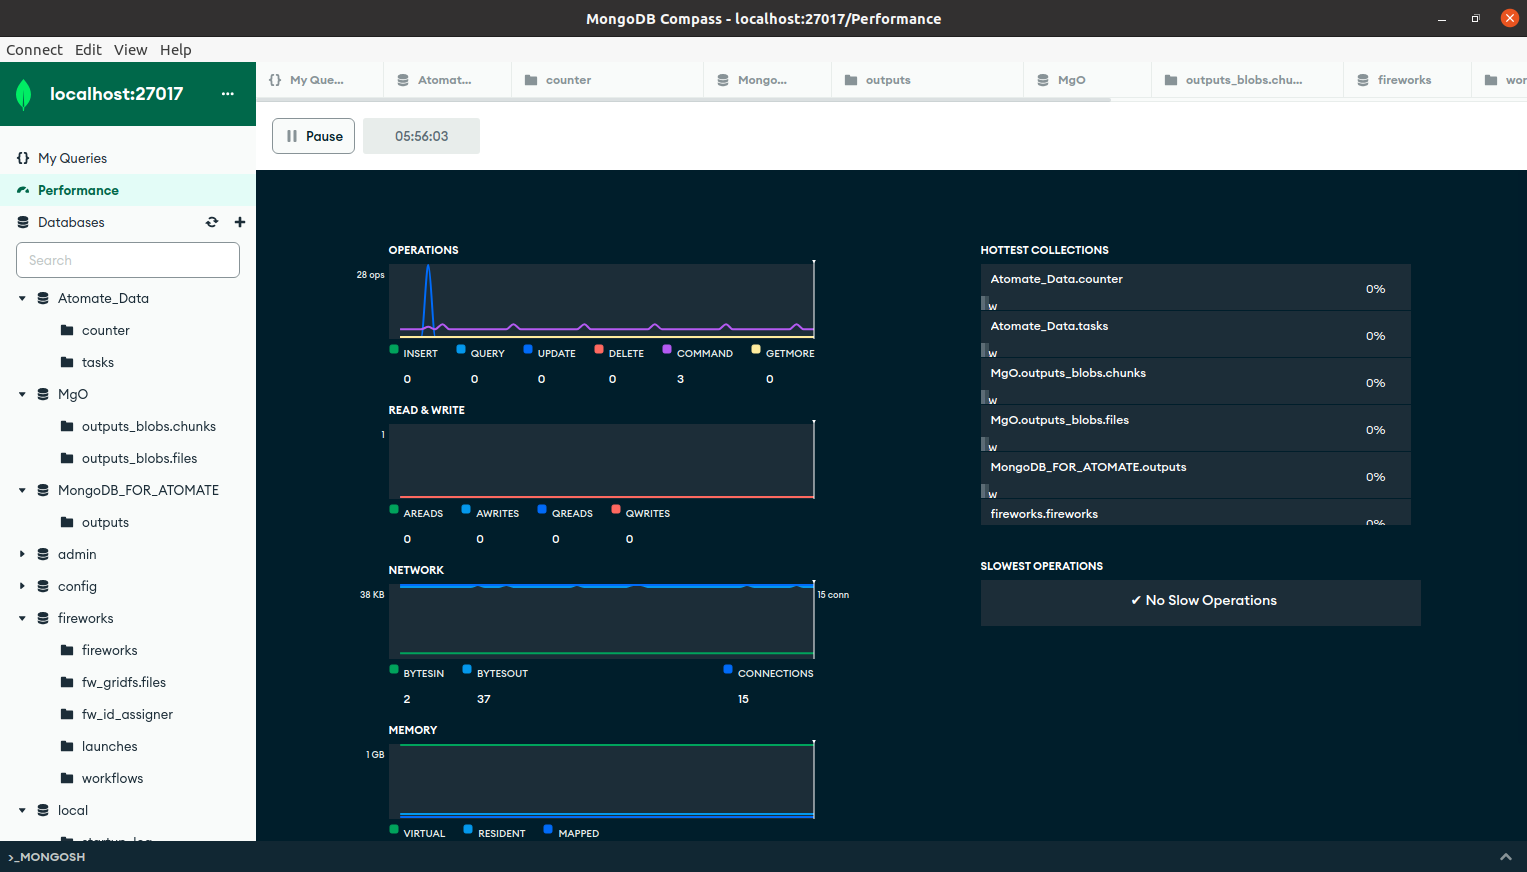
\includegraphics[height=2.35in,width=4.05in,viewport=0 0 1527 872,clip]{Figures/Database_Materials-3.png}
%\caption{\tiny \textrm{Pseudopotential for metallic sodium, based on the empty core model and screened by the Thomas-Fermi dielectric function.}}%(与文献\cite{EPJB33-47_2003}图1对比)
\label{DataBase_Materials-3}
\end{figure}
}

\frame
{
	\frametitle{数据的硬件基础:~高性能计算资源}
全国高校计算联盟:~资源类型
\begin{figure}[h!]
\vspace*{-0.15in}
\centering
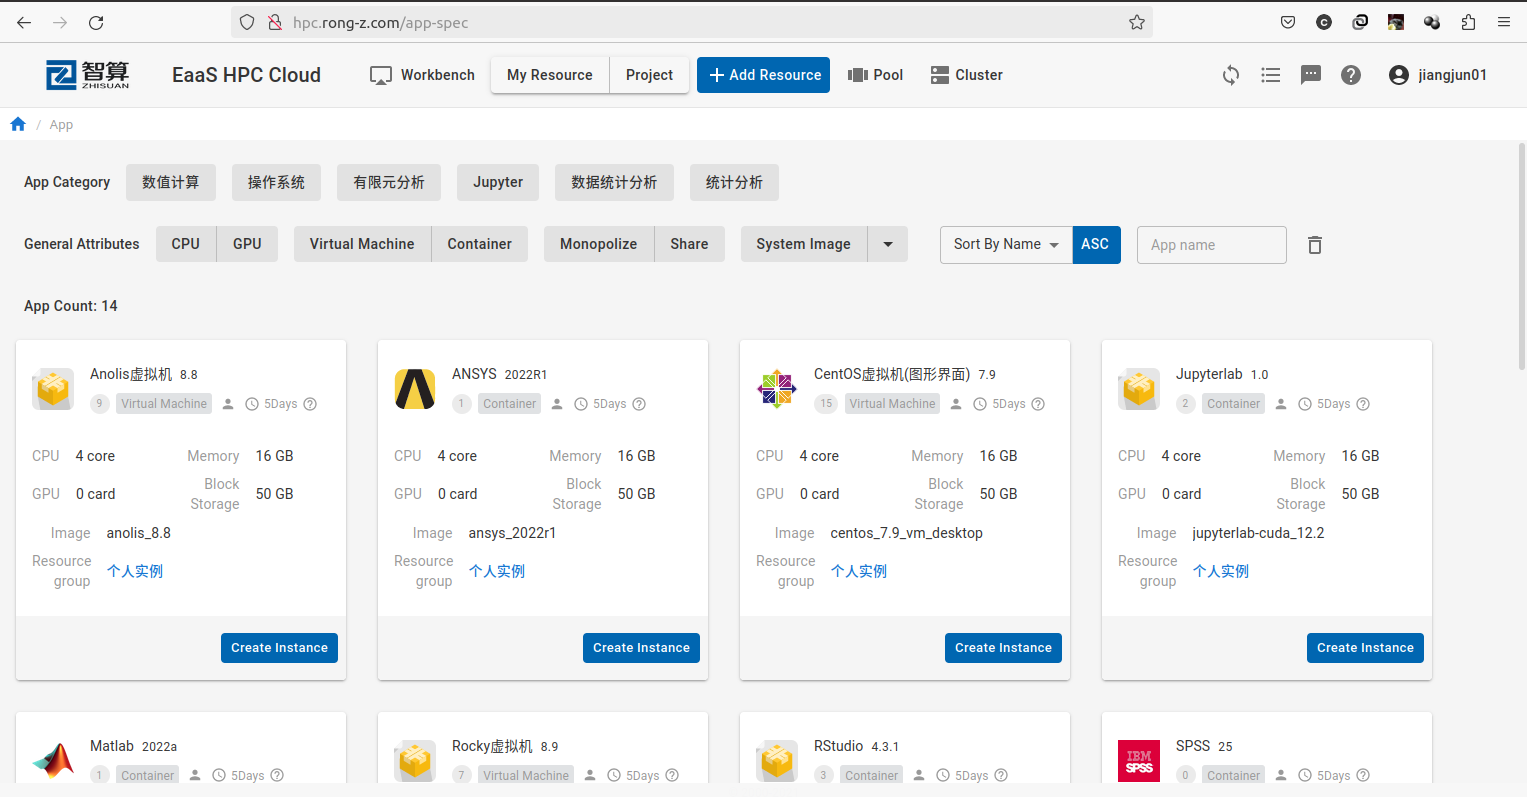
\includegraphics[height=2.15in,width=4.05in,viewport=0 0 1527 797,clip]{Figures/Eaas-HPC-Cloud.png}
%\caption{\tiny \textrm{Pseudopotential for metallic sodium, based on the empty core model and screened by the Thomas-Fermi dielectric function.}}%(与文献\cite{EPJB33-47_2003}图1对比)
\label{Eaas-HPC-Cloud}
\end{figure}
}

\frame
{
	\frametitle{数据的硬件基础:~计算资源}
全国高校计算联盟:~资源配额
\begin{figure}[h!]
\vspace*{-0.15in}
\centering
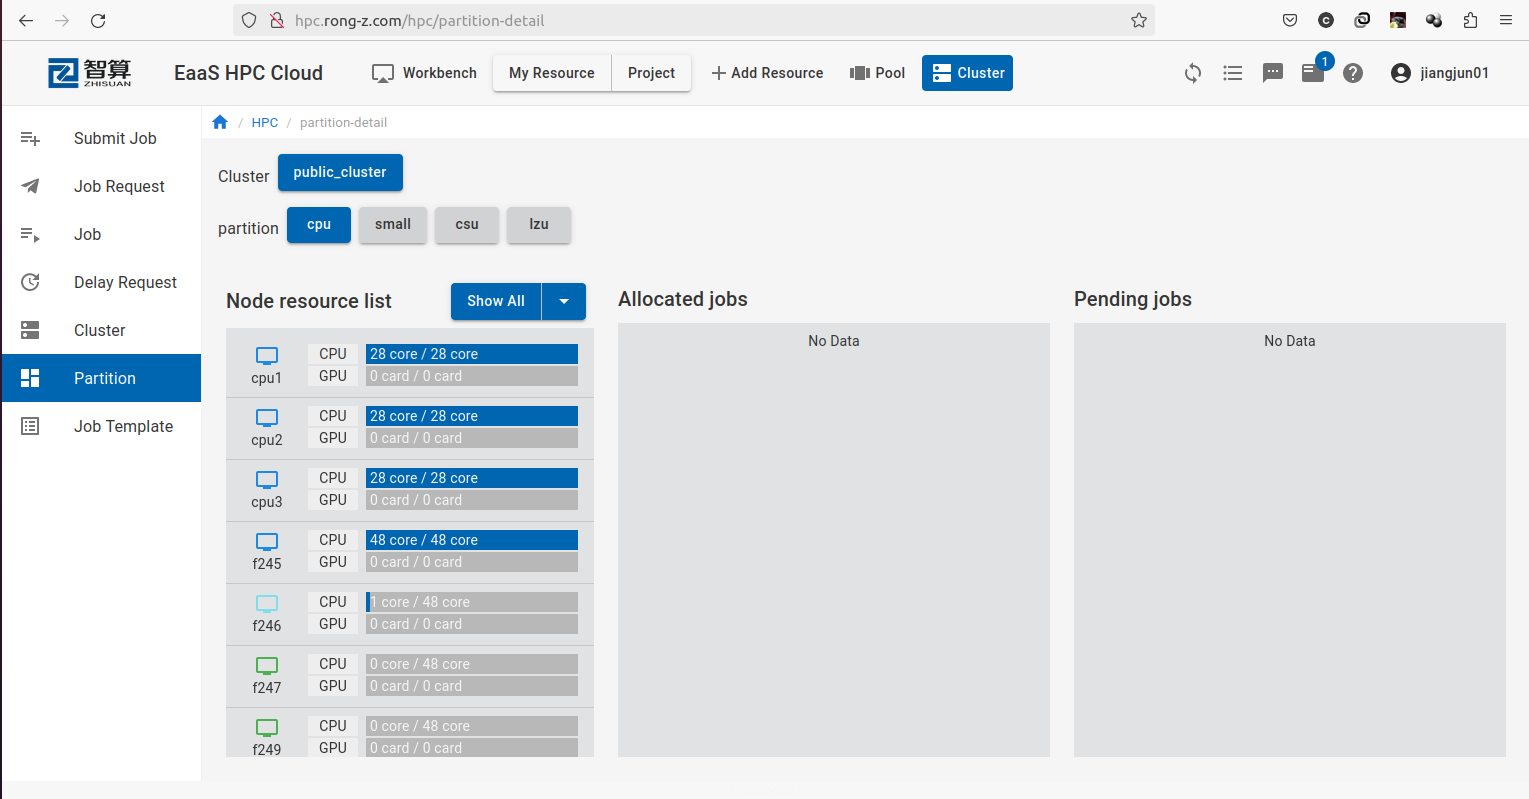
\includegraphics[height=2.15in,width=4.05in,viewport=0 0 1529 799,clip]{Figures/Eaas-HPC-Cloud-resource.png}
%\caption{\tiny \textrm{Pseudopotential for metallic sodium, based on the empty core model and screened by the Thomas-Fermi dielectric function.}}%(与文献\cite{EPJB33-47_2003}图1对比)
\label{Eaas-HPC-Cloud-resource}
\end{figure}
}

\frame
{
	\frametitle{材料计算软件发展现状}
\begin{figure}[h!]
\vspace*{-0.16in}
\centering
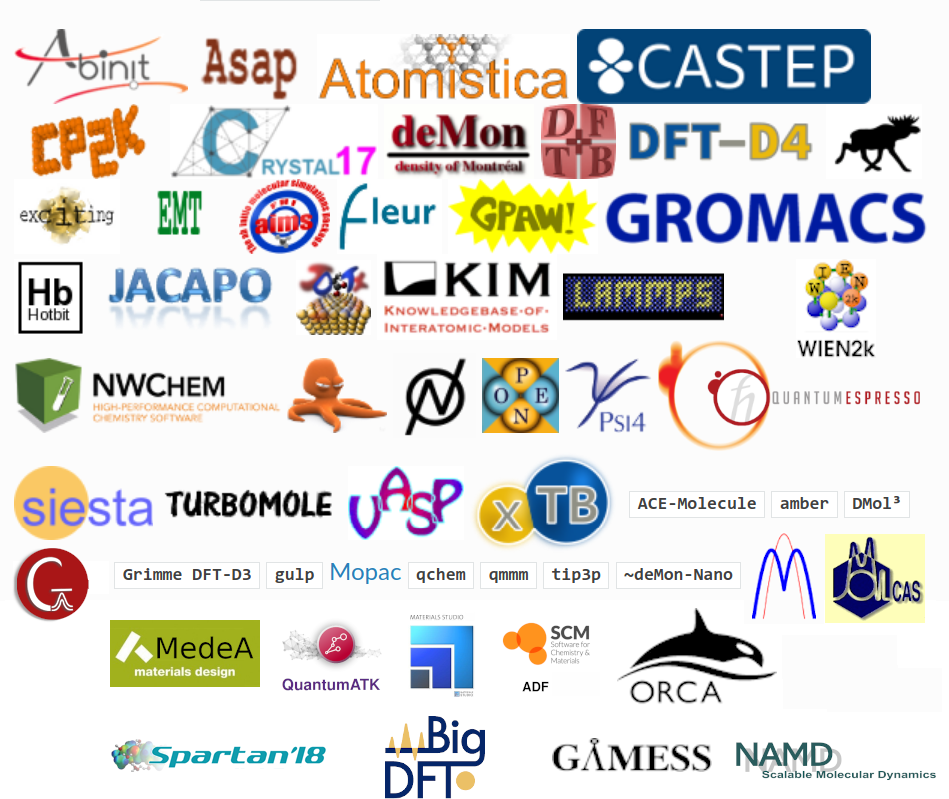
\includegraphics[width=3.30in]{Figures/Softwares_logo.png}
%\caption{\tiny \textrm{Pseudopotential for metallic sodium, based on the empty core model and screened by the Thomas-Fermi dielectric function.}}%(与文献\cite{EPJB33-47_2003}图1对比)
\label{Softwares}
\end{figure}
}

\frame
{
	\frametitle{\textrm{VASP}:~第一原理计算软件的代表}
	{\fontsize{8.2pt}{7.2pt}\selectfont{
	作为第一性原理计算的商用软件,\textrm{VASP}已成为计算材料学领域应用最广泛的软件之一。全球绝大多数超算中心都安装了\textrm{VASP},据统计,\textrm{VASP}软件的作业机时占用全球总机时的12$\sim$20\%,但由于其%类似于linpack软件,
属于重型浮点计算密集型应用,实际耗电量占比则高达30$\sim$50\%
\vskip 3pt
	\begin{itemize}
		\item 提供了多种电子结构和原子受力的优化算法(\textrm{SD}、\textrm{CG}、\textrm{RMM-DIIS}等)%\\
%			用户可以通过控制文件\textcolor{blue}{\textrm{INCAR}}的参数调控来选择
		\item 与同类型软件相比,\textrm{VASP}有着优异的并行能力
\begin{figure}[h!]
	\vspace{-0.15in}
\centering
%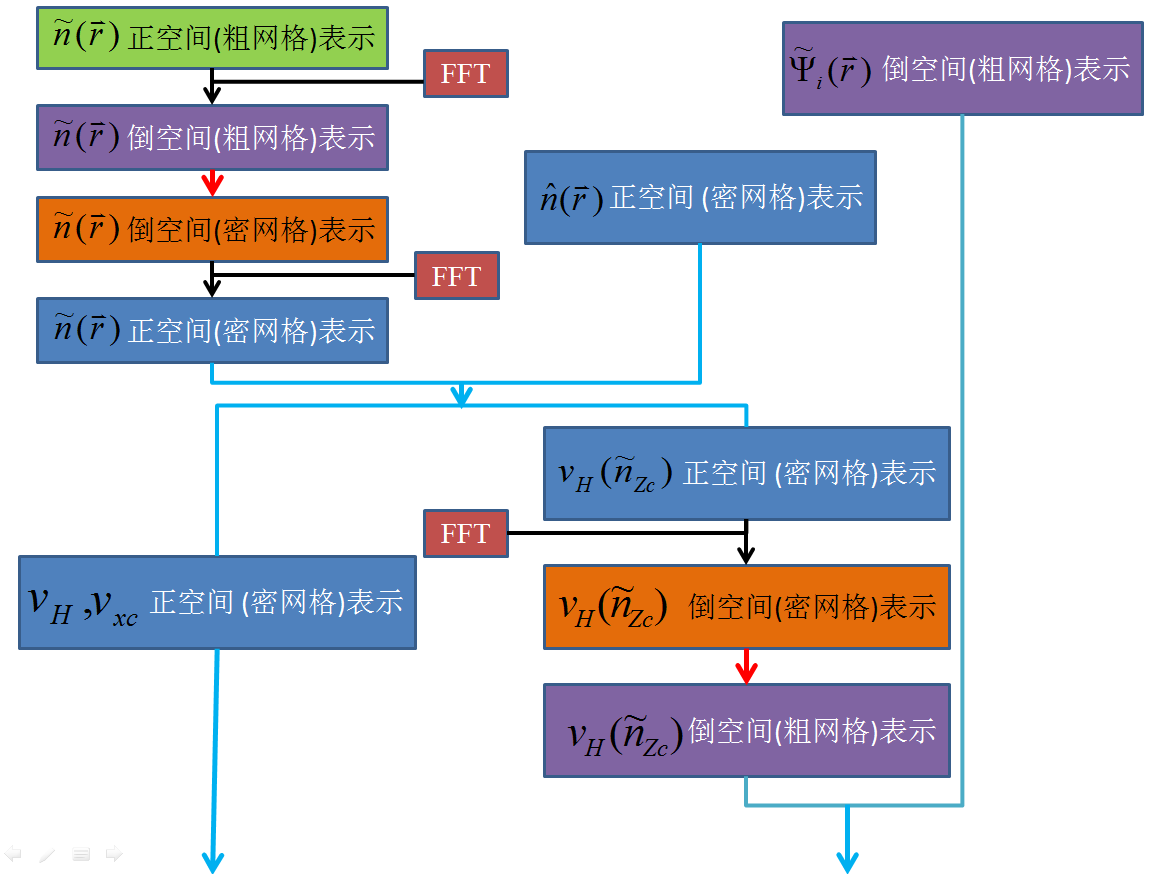
\includegraphics[height=2.7in,width=4.0in,viewport=0 0 1180 875,clip]{Figures/dual_grid.png}
%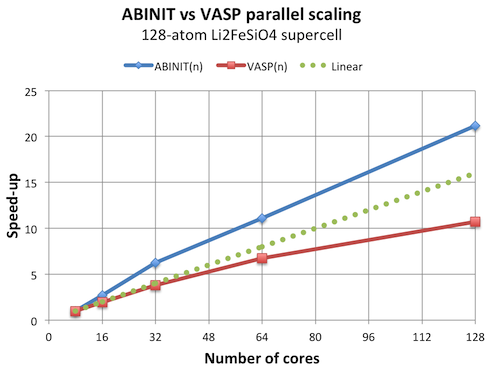
\includegraphics[height=1.55in,width=1.95in,viewport=0 0 240 200,clip]{Figures/VASP-abinit_Li128-1.png}
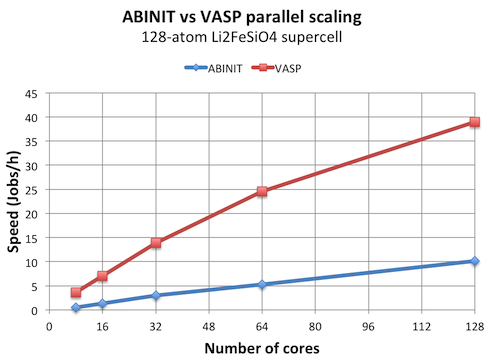
\includegraphics[height=1.55in,width=1.95in,viewport=0 0 240 200,clip]{Figures/VASP-abinit_Li128-2.png}
\caption{\tiny \textrm{The comparison of parallel scaling for ABINIT vs VASP.}}%(与文献\cite{EPJB33-47_2003}图1对比)
\label{ABINIT_vs_VASP}
\end{figure} 
%		\item 提供了基于\textrm{PAW}方法适用性广泛的原子数据集文件\textrm{POTCAR}
	\end{itemize}}}
%			\textcolor{magenta}{有必要探索新的并行和优化策略来提升\textrm{VASP}的计算性能}
}

\frame
{
	\frametitle{\textrm{VASP}的基础:~原子数据集}
	{\fontsize{7.2pt}{7.2pt}\selectfont{
	\begin{itemize}
		\item \textrm{POTCAR}是\textrm{VASP}实现材料精确计算的重要保证%\\
%			同样都应用\textrm{PAW}方法,\textcolor{blue}{公认\textrm{VASP}较\textrm{QE}、\textrm{ABINIT}等软件的计算精度要高}
%		\item \textrm{POTCAR}数据生成依赖较多的可调参数\\
%			包括能量参数$\varepsilon_l$、多种截断半径$r_c$、$r_{\mathrm{vloc}}$、$r_{\mathrm{shape}}$、$r_{\mathrm{core}}$
		\item \textcolor{red}{\textrm{POTCAR}数据生成代码是\textrm{VASP}中唯一没有公开的}
%		\item 用\textrm{VASP}模拟极端条件下材料物性的能力,受到\textrm{POTCAR}数据的制约
	\end{itemize}}}
\begin{figure}[h!]
\centering
\vskip -0.5in
\includegraphics[width=1.5in,height=2.7in,viewport=0 0 350 550, angle=-90, clip]{Figures/WAE-data.eps}
\vskip -0.2in
\includegraphics[height=2.7in,width=1.5in,viewport=0 0 350 550, angle=-90, clip]{Figures/WPS-data.eps}
\caption{\tiny \textrm{The partial wave function.}}%(与文献\cite{EPJB33-47_2003}图1对比)
\label{Wave_Function}
\end{figure}
}

\frame
{
	\frametitle{\textrm{PAW}原子数据集:~\textrm{core~density}}
	\textcolor{blue}{构造赝芯电荷密度$\tilde n_c$}:~在截断半径$r_{\mathrm{core}}$内的定义为
	$$\sum_{i=1,2}B_i\dfrac{\sin(q_ir)}r\quad r<r_{\mathrm{core}}$$
	调节系数$q_i$和$B_i$使得赝芯电荷密度$\tilde n_c(r)$在截断半径$r_{\mathrm{core}}$处的两阶导数连续
\begin{figure}[h!]
\vskip -0.5in
\centering
\hspace*{-0.1in}
\includegraphics[width=1.5in,height=2.35in,viewport=0 0 350 550, angle=-90, clip]{Figures/CORE-data.eps}
\hspace*{-0.7in}
\includegraphics[height=2.35in,width=1.5in,viewport=0 0 350 550, angle=-90, clip]{Figures/PCORE-data.eps}
\caption{\tiny \textrm{The core density.}}%(与文献\cite{EPJB33-47_2003}图1对比)
\label{core_density_Function}
\end{figure}
}

\frame
{
	\frametitle{\textrm{PAW}原子数据集:~$\mathrm{v}_{e\!f\!f}(r)$与$\tilde{\mathrm{v}}_{e\!f\!f}(r)$}
	\textcolor{blue}{原子局域有效势$\mathrm{v}_{e\!f\!f}^a$}
\begin{figure}[h!]
%\vskip -0.5in
\vskip -0.17in
\centering
%\includegraphics[width=1.6in,height=2.7in,viewport=0 0 300 460, angle=-90, clip]{Figures/POTAE-data.eps}
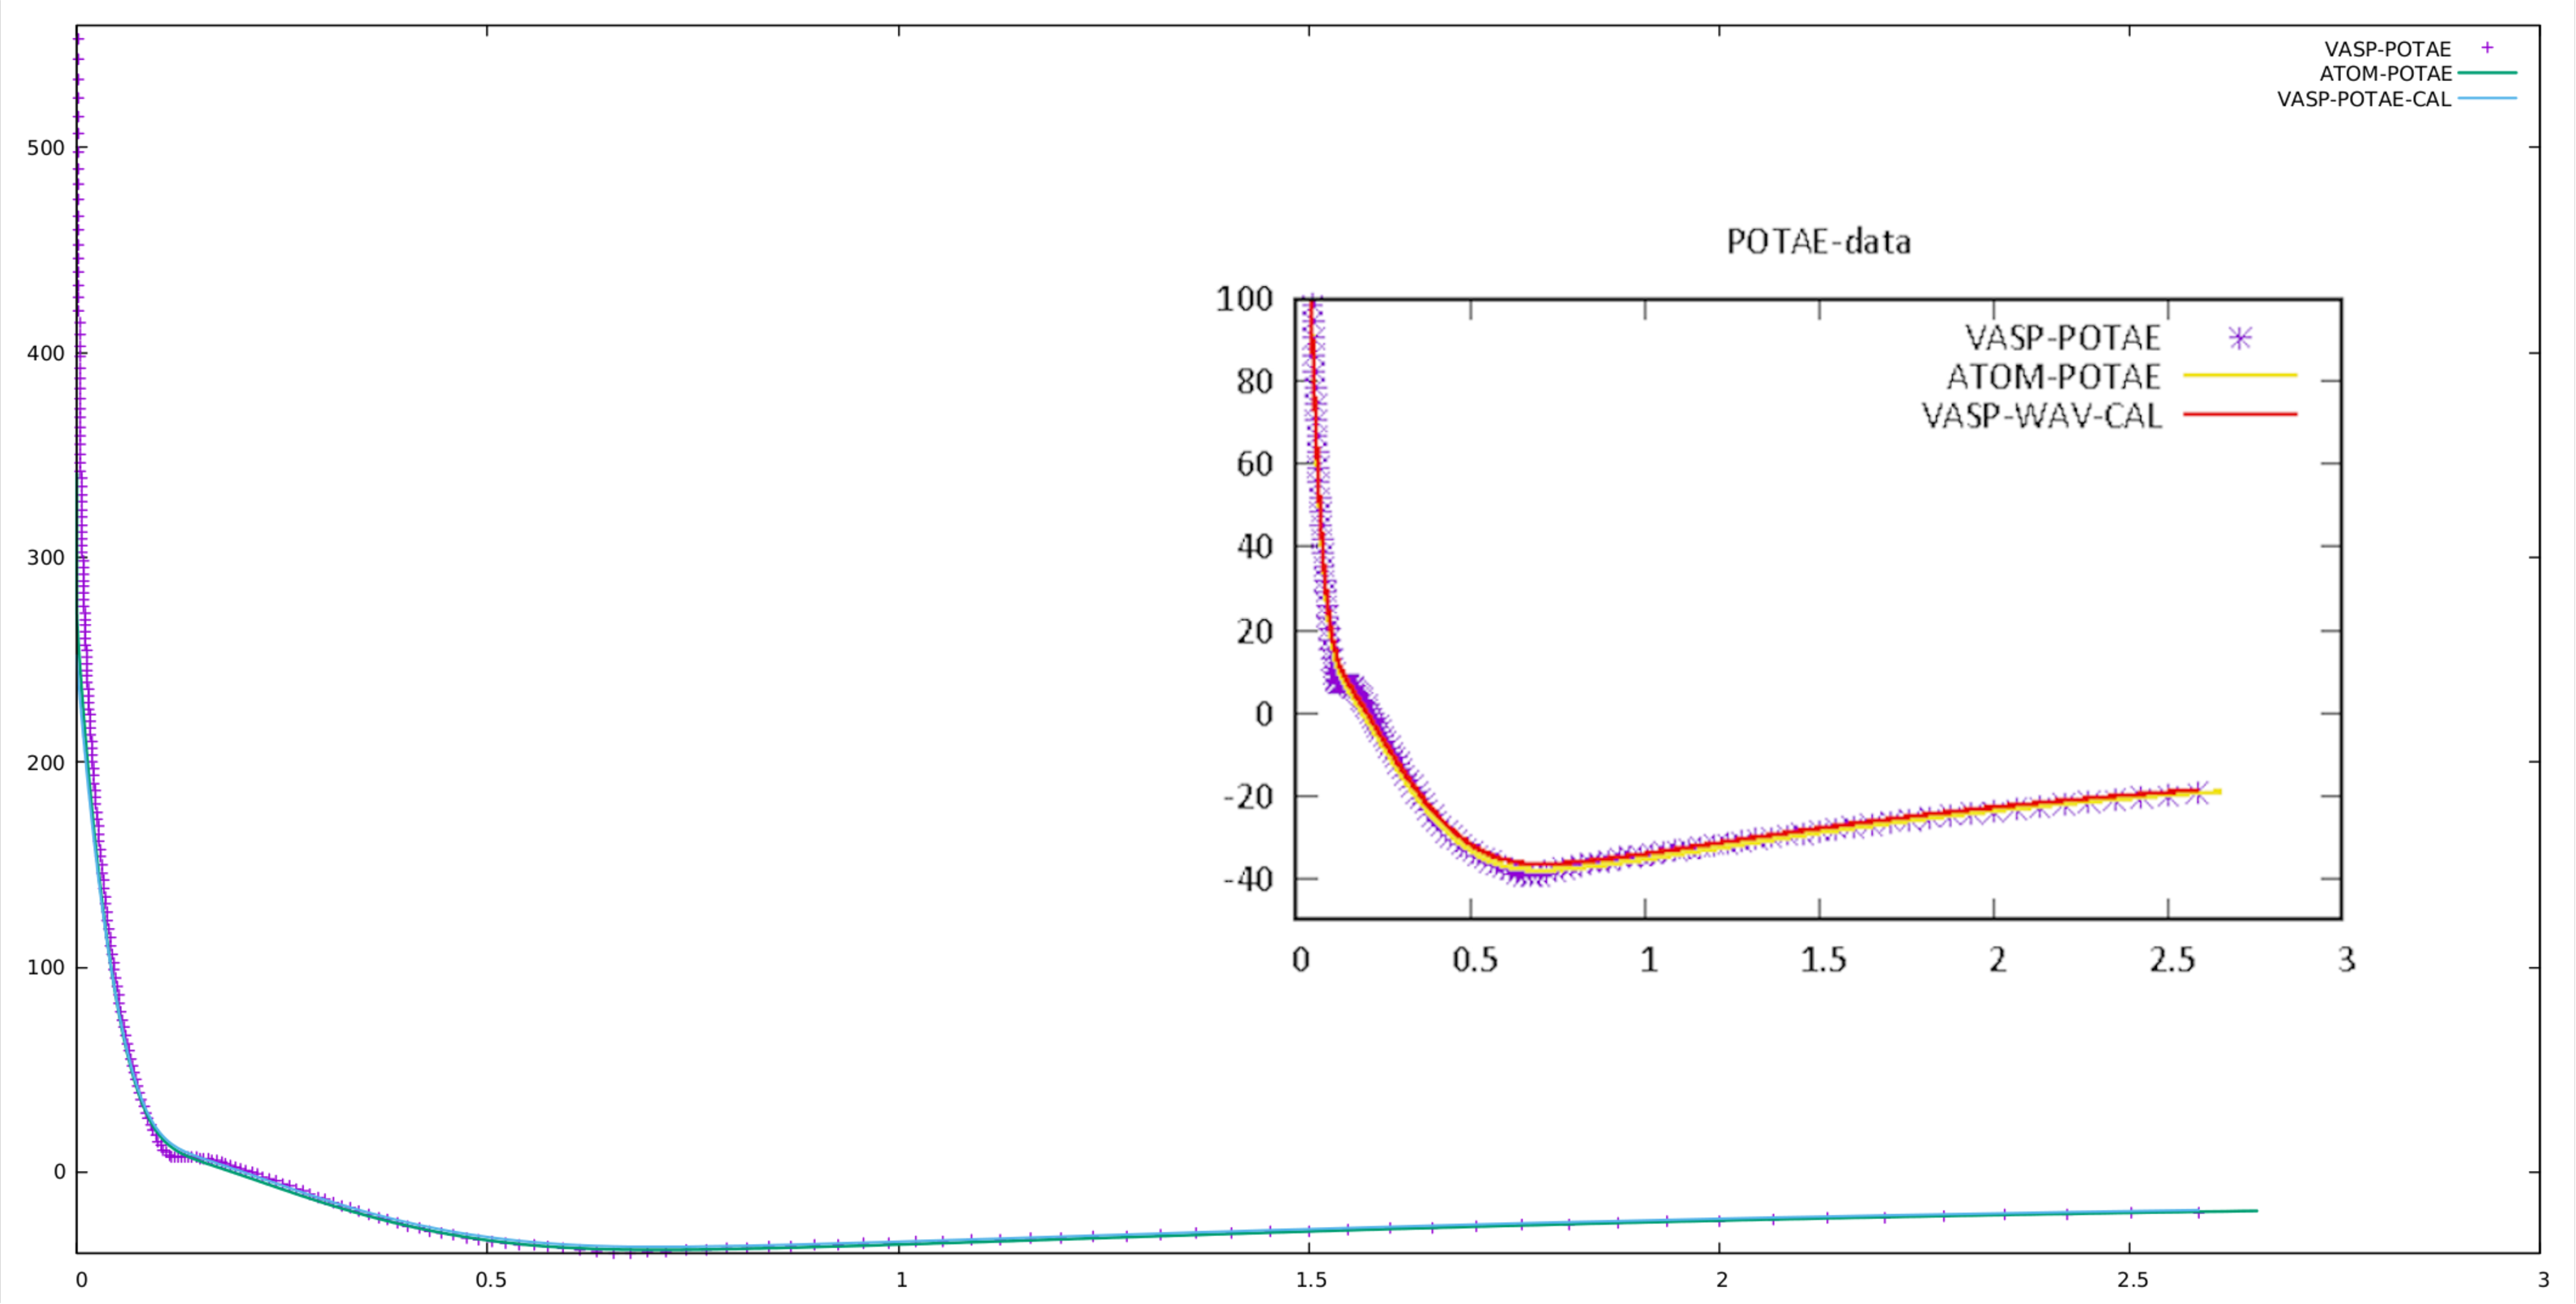
\includegraphics[width=2.5in,height=1.2in,viewport=0 0 1600 800, clip]{Figures/POTAE-full-dat.pdf}
\caption{\tiny \textrm{The local atomic effective-Potential.}}%(与文献\cite{EPJB33-47_2003}图1对比)
\label{local_atomic_PP}
\end{figure}
	\textcolor{blue}{构造原子局域赝势$\tilde v_{e\!f\!f}^a$}%(\textcolor{red}{为防止\textrm{ghost band}})
	:%\\
	(在截断半径$r_{\mathrm{loc}}$内的定义)
	$$\tilde v_{e\!f\!f}^a=A\dfrac{\sin(q_{loc}r)}r\quad r<r_{\mathrm{loc}}$$
	其中$q_{loc}$和$A$要求局域赝势在截断半径$r_{\mathrm{loc}}$处连续到一阶导数
}

\frame
{
	\frametitle{\textrm{PAW}原子数据集:~$\mathrm{v}_H[\tilde n_{Zc}]$}
	局域离子赝势$v_H[\tilde n_{Zc}]$可由原子局域赝势去屏蔽得到
	$$v_H[\tilde n_{Zc}]=\tilde v_{e\!f\!f}^a-v_H[\tilde n_a^1+\hat n_a]-v_{\mathrm{XC}}[\tilde n_a^1+\hat n_a+\tilde n_c]$$
\begin{figure}[h!]
\vskip -0.5in
\centering
\hspace*{-0.1in}
\includegraphics[width=1.5in,height=2.35in,viewport=0 0 350 550, angle=-90, clip]{Figures/POTPS-data.eps}
\hspace*{-0.7in}
\includegraphics[height=2.35in,width=1.5in,viewport=0 0 350 550, angle=-90, clip]{Figures/POTPSC-data.eps}
\caption{\tiny \textrm{The pseudo-potential and local ionic pseudo-potential.}}%(与文献\cite{EPJB33-47_2003}图1对比)
\label{pseudo_potential}
\end{figure}
}

\frame
{
	\frametitle{\textrm{PAW}原子数据集:~$\tilde{n}_{\mathrm G}$}
	局域离子赝势$\tilde{n_{\mathrm G}}$可由原子局域赝密度的\textrm{FFT}得到
\begin{figure}[h!]
\vskip -0.2in
\centering
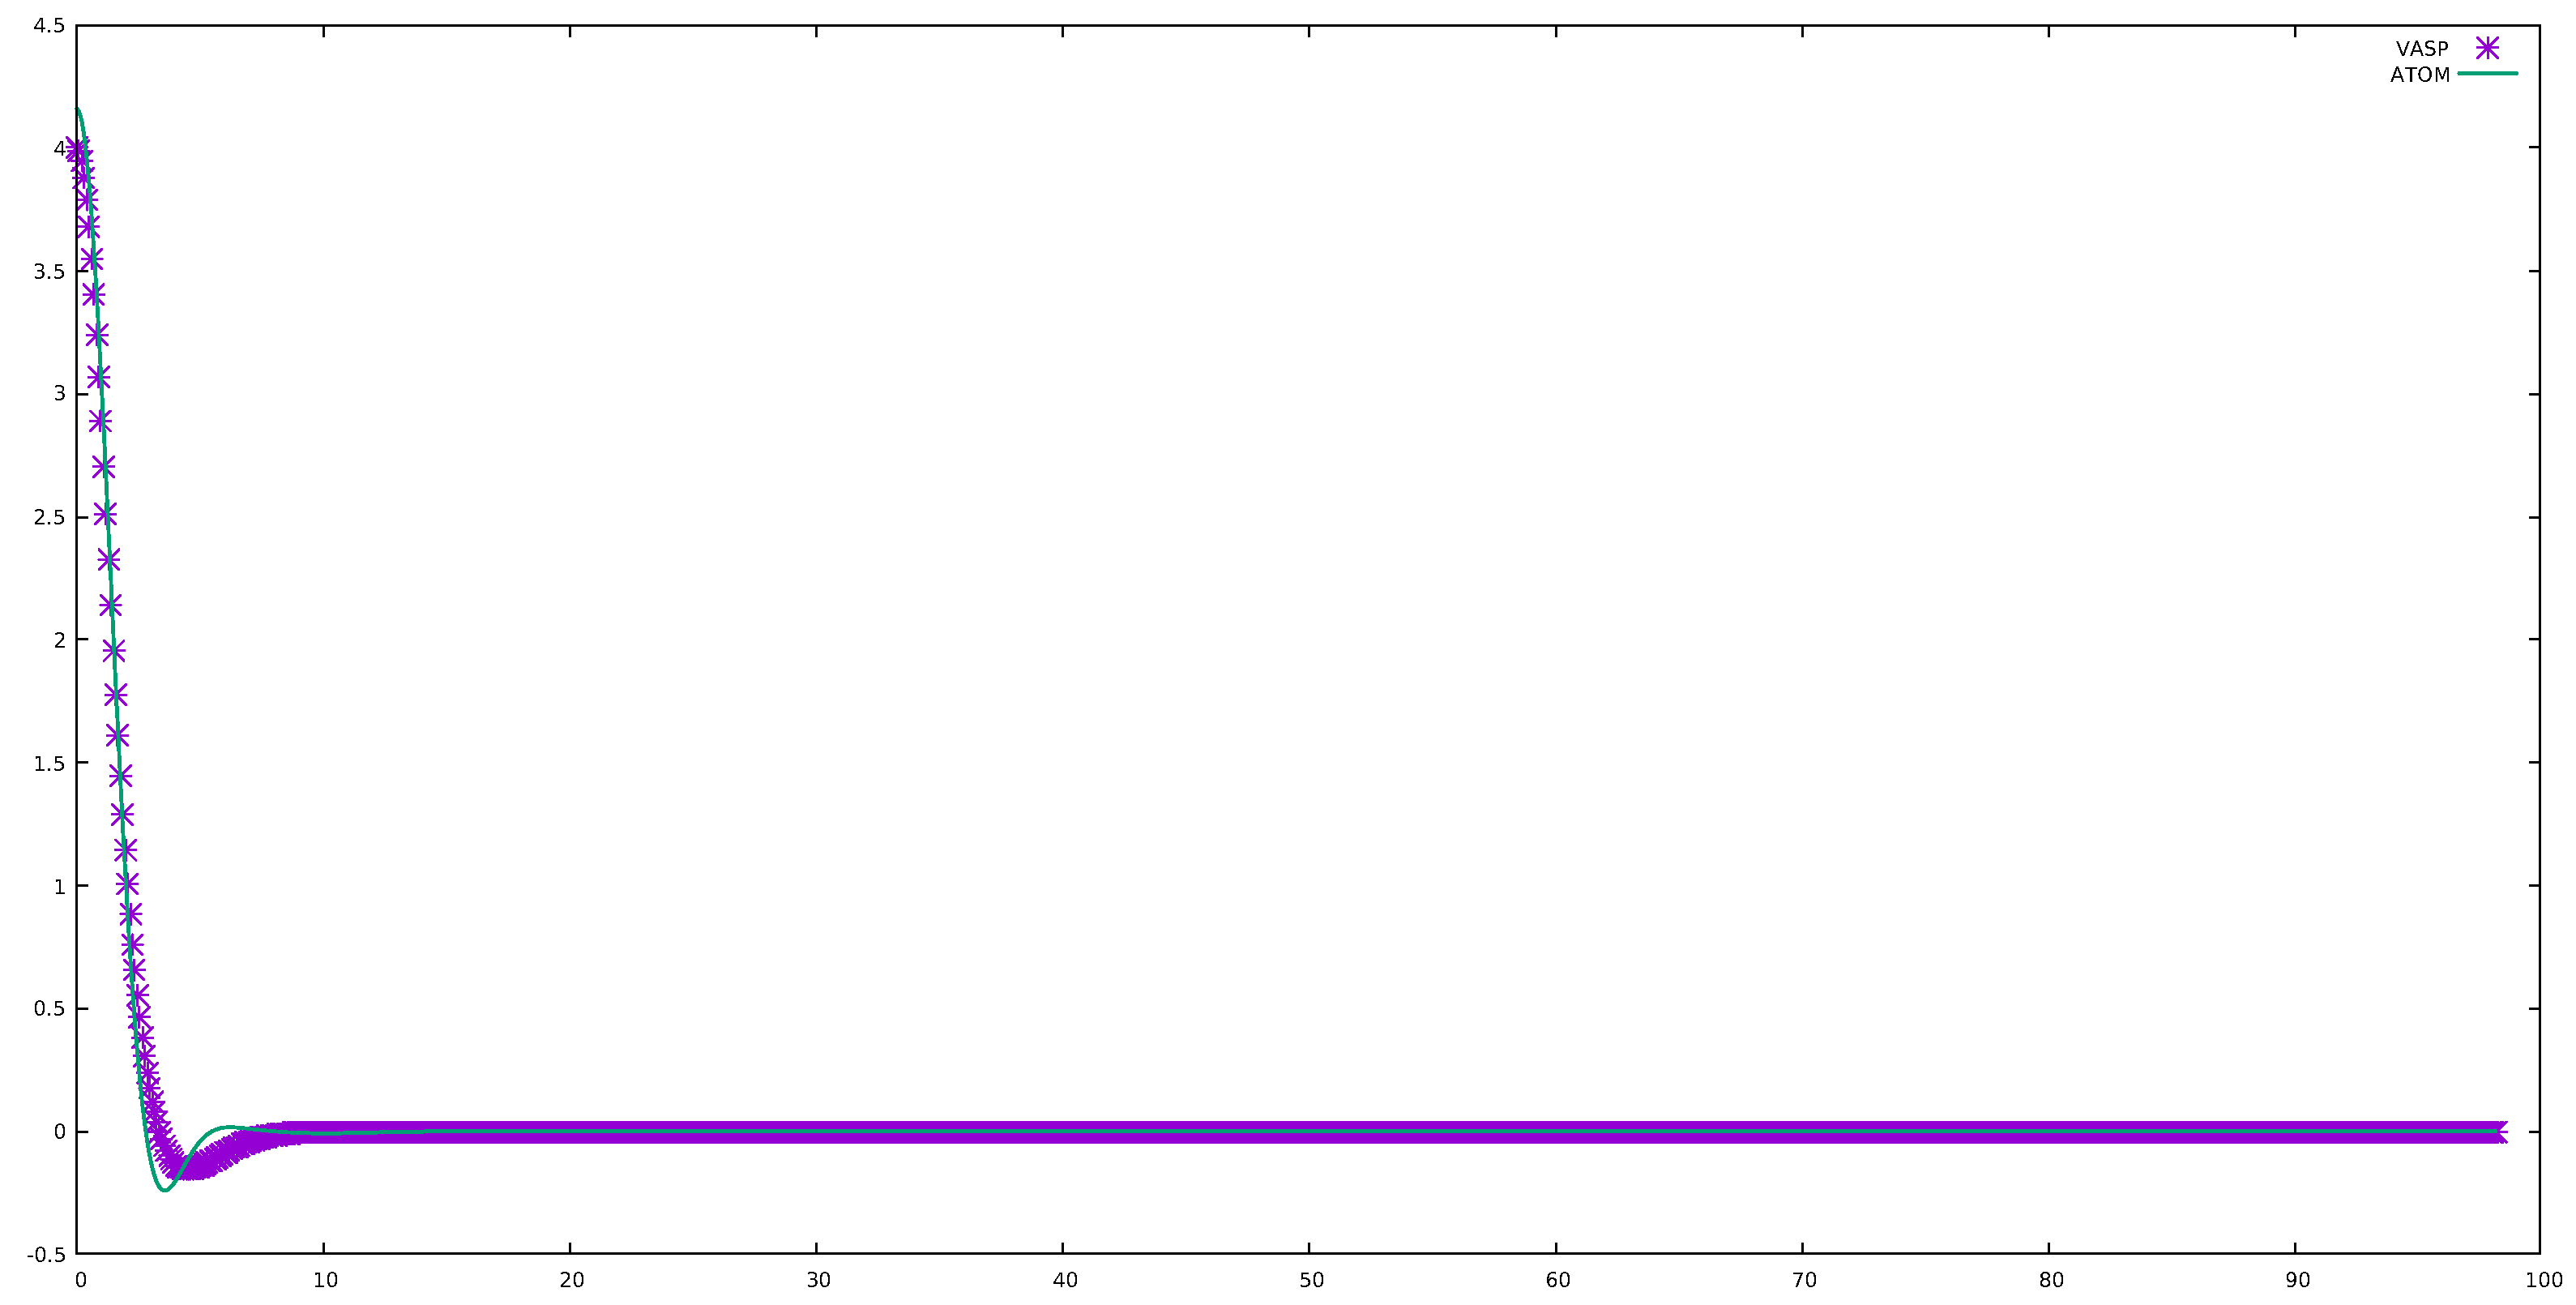
\includegraphics[width=4.0in,height=2.35in,viewport=0 0 1530 850, clip]{Figures/PSRHO_G-dat.pdf}
\caption{\tiny \textrm{The pseudo-density in reciprocal space.}}%(与文献\cite{EPJB33-47_2003}图1对比)
\label{pseudo_density_in_reciprocal-space}
\end{figure}
}

\frame
{
	\frametitle{\textrm{PAW}原子数据集:~$\mathrm{v}_{\mathrm G}[\tilde n_{Zc}]$}
	局域离子赝势在倒空间的表示$v_{\mathrm G}[\tilde n_{Zc}]$可由原子去屏蔽局域赝势的\textrm{FFT}得到
\begin{figure}[h!]
\vskip -0.2in
\centering
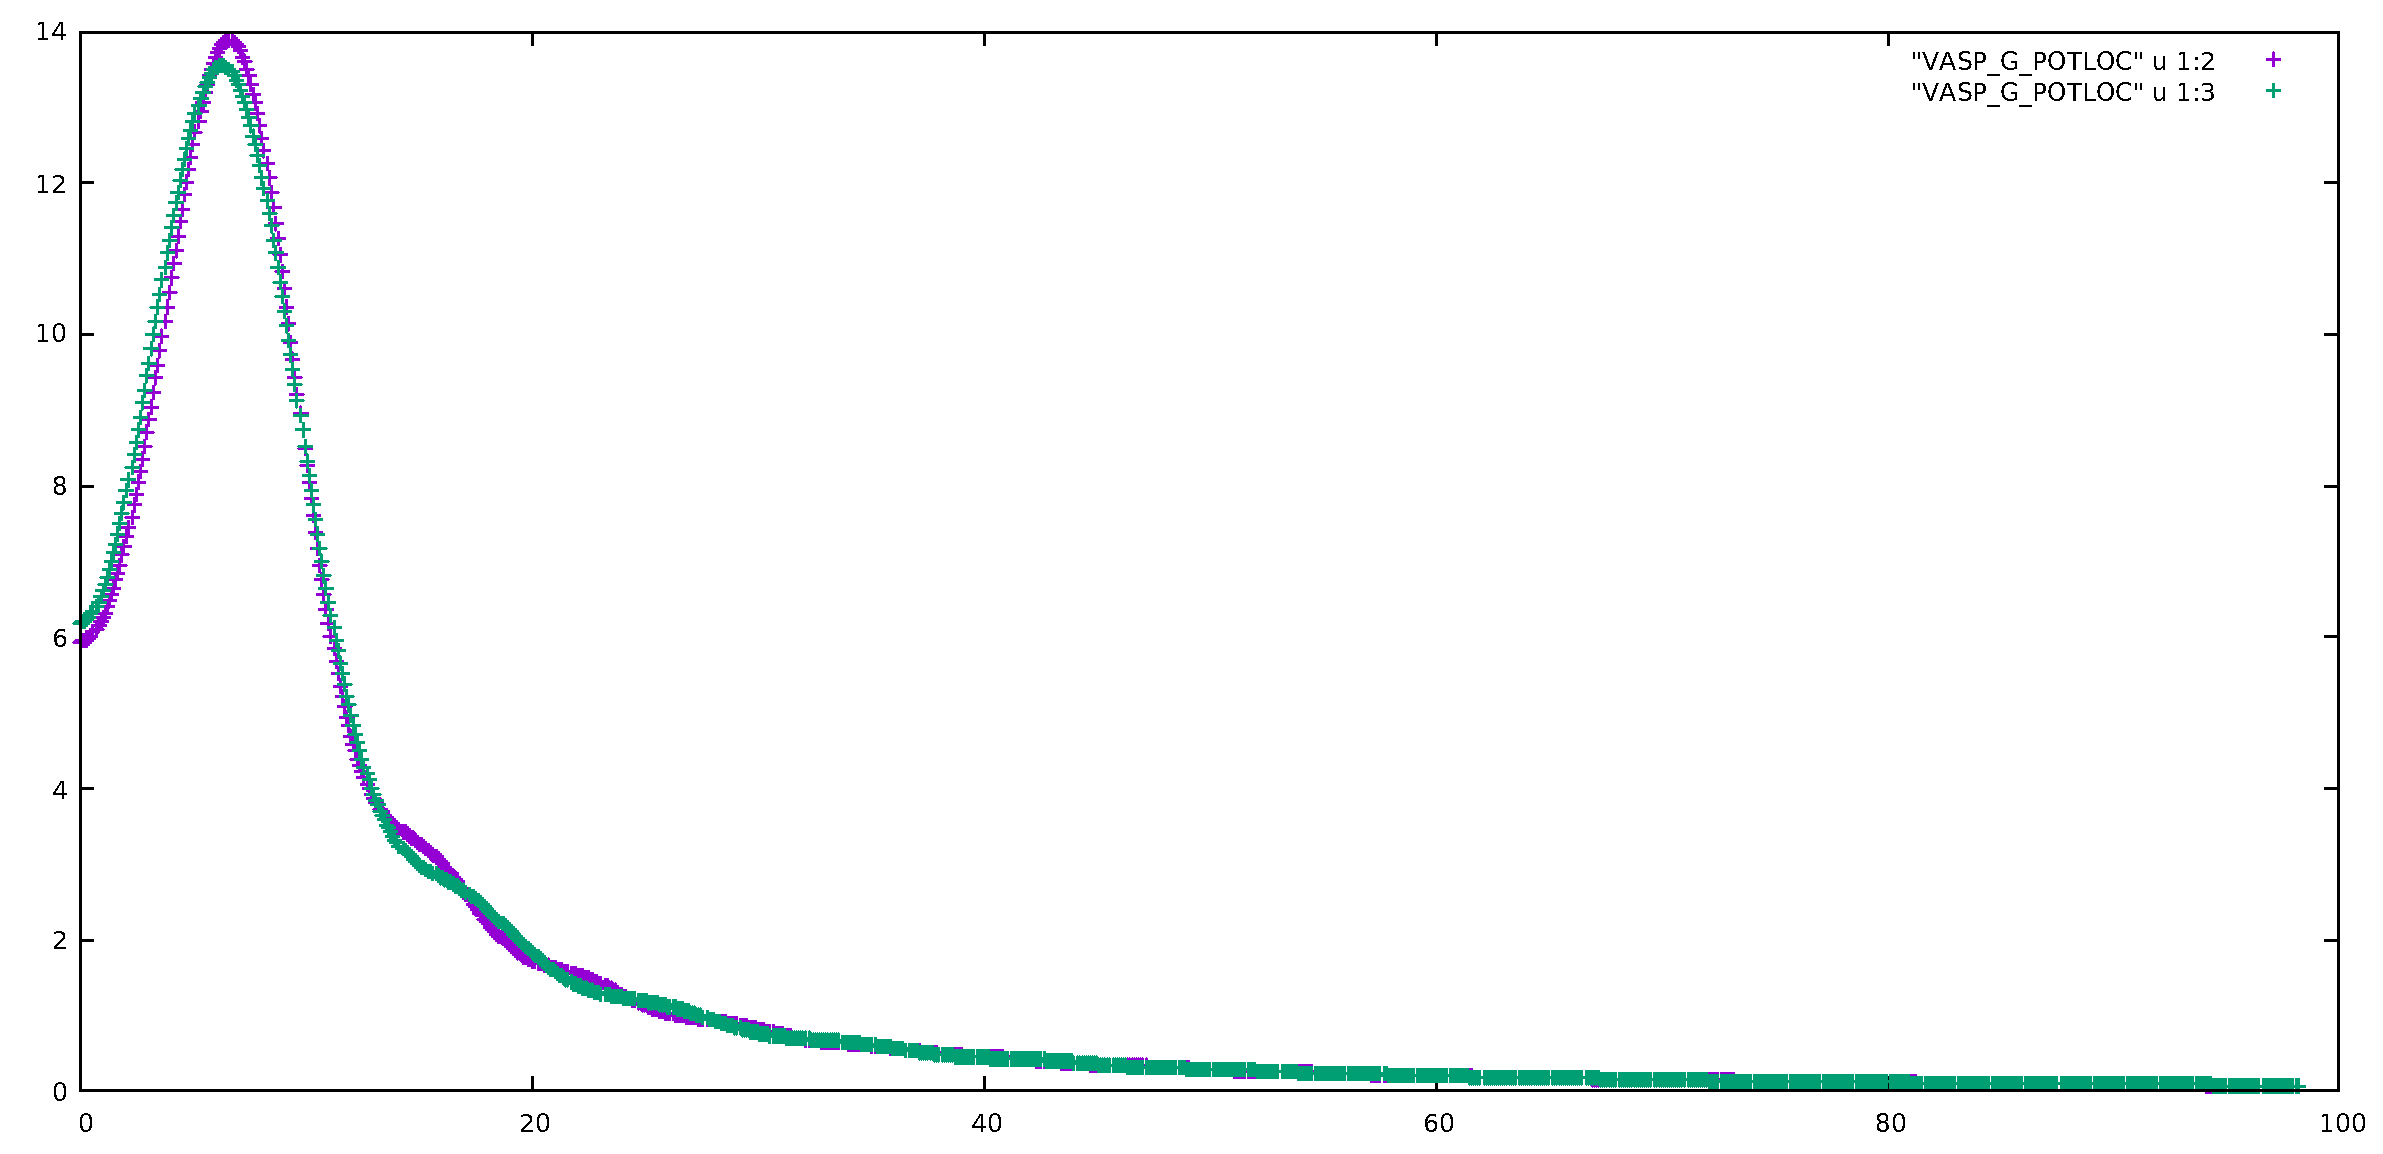
\includegraphics[width=4.0in,height=2.35in,viewport=0 0 1150 650, clip]{Figures/POT_G-dat.pdf}
\caption{\tiny \textrm{The local ionic pseudo-potential in reciprocal space.}}%(与文献\cite{EPJB33-47_2003}图1对比)
\label{pseudo_potential_in_reciprocal-space}
\end{figure}
}

%-----------------------------------------------------------------------------------------------------------------------------------------------------------------------%
\frame
{
	\frametitle{跨尺度计算的需求:~合金材料}
\begin{figure}[h!]
\vspace*{-0.20in}
\centering
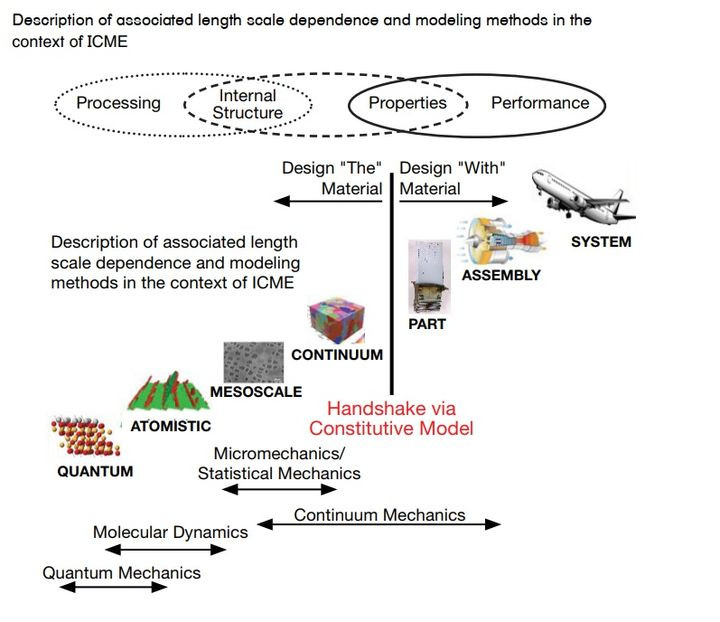
\includegraphics[height=2.80in,width=3.35in,viewport=0 0 170 150,clip]{Figures/Multi_Scale-6.jpg}
%\caption{\tiny \textrm{Pseudopotential for metallic sodium, based on the empty core model and screened by the Thomas-Fermi dielectric function.}}%(与文献\cite{EPJB33-47_2003}图1对比)
\label{Alloy-Multi_Scale}
\end{figure}
}

\frame
{
	\frametitle{跨尺度计算的需求:~电池材料}
\begin{figure}[h!]
\vspace*{-0.13in}
\centering
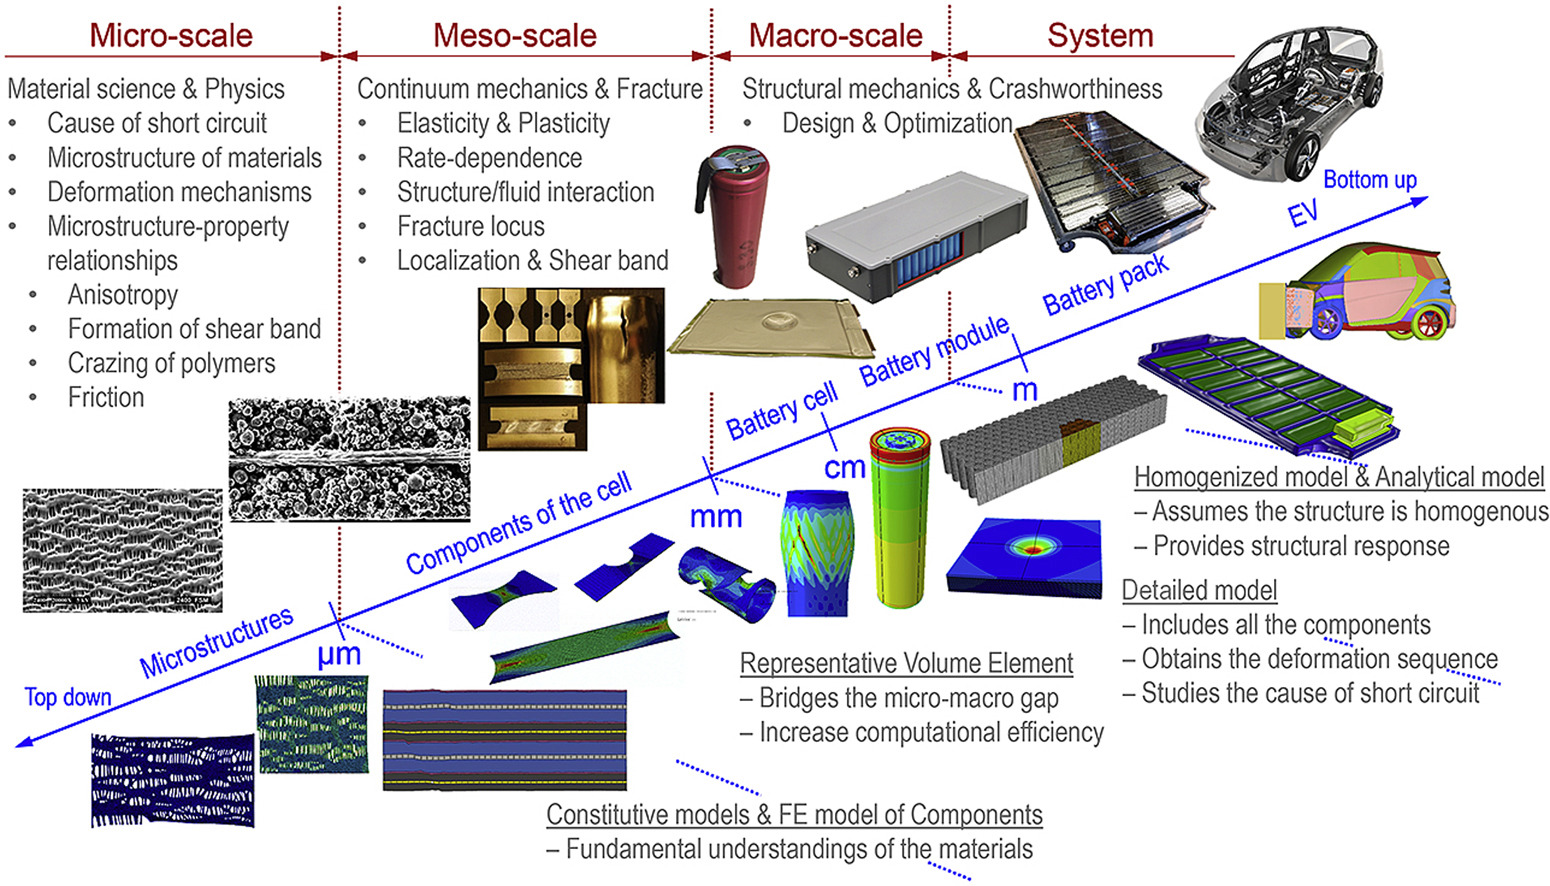
\includegraphics[height=2.50in,width=4.05in,viewport=0 0 224 125,clip]{Figures/Multiple_scales-Battery_cell.jpg}
%\caption{\tiny \textrm{Pseudopotential for metallic sodium, based on the empty core model and screened by the Thomas-Fermi dielectric function.}}%(与文献\cite{EPJB33-47_2003}图1对比)
\label{Battery_Cell-Multi_Scale}
\end{figure}
}

\frame
{
	\frametitle{材料科学的梦想:~\textrm{AI for Mateials}}
\begin{figure}[h!]
\vspace*{-0.18in}
\centering
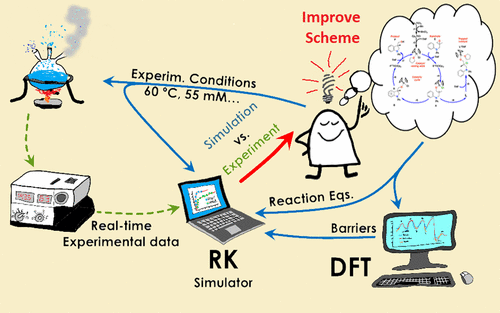
\includegraphics[height=2.55in,width=4.05in]{Figures/Schematic_Material-Design.png}
\caption{\tiny \textrm{AI for materials:~I~Have~A~Dream.}}%(与文献\cite{EPJB33-47_2003}图1对比)
%\caption{\tiny \textrm{Pseudopotential for metallic sodium, based on the empty core model and screened by the Thomas-Fermi dielectric function.}}%(与文献\cite{EPJB33-47_2003}图1对比)
\label{Schematic_Material-Design}
\end{figure} 
}

